%%%%%%%%%%%%%%%%%%%%%%%%%%%%%%%%%%%%%%%%%%%%%%%%%%%%%%%%%%%%%%%%%%%%%%%%%%%%%%%%
% simulation.tex: Chapter on MC production:
%%%%%%%%%%%%%%%%%%%%%%%%%%%%%%%%%%%%%%%%%%%%%%%%%%%%%%%%%%%%%%%%%%%%%%%%%%%%%%%%
\chapter{Experiment Simulation}
\label{simulation_chapter}
The complex, quantum nature of high energy particle interactions within the detector generally makes direct computation of the expected behavior of collision products extremely difficult.
To avoid this issue, typical analyses using the CMS detector rely on detailed simulations of the physics processes and particle reconstruction within each event to compare with observations in data.
The standard tool used to produce these simulations is the Monte Carlo (MC) method, where physics processes of interest and their interactions with the detector are simulated using random number generators to individually produce full events.

By creating large numbers of individual events, the underlying distributions of their observables can be determined and compared to data, and modifications to the available physics can be added to find the expected impact of any given physics model and determine whether its signature is present in data.
Because of the underlying uncertainties and assumptions required to create these simulated events, careful validation of their behavior through comparisons with data in control regions is necessary to determine whether any observed differences are due to new physics or are artifacts produced by the simulation process.

Many inputs are required to produce accurate simulations of CMS events.
First, the initial proton collision must be simulated for the process of interest, as well as its resulting decay into observable particles, generally referred to as the 'generation' step.
Next, the propagation, interactions, and decays of the initial collision products in the CMS detector must be simulated, a fundamentally quantum and probabilistic process, as well as the deposits in the detector from these interactions, which together are known as the 'simulation' step.
Lastly, the response of the active detector elements to these particles is simulated and transformed into the digital formats used in the real detector so that identical reconstruction algorithms can be applied to simulated and data events, known as the 'digitization' step.

In this section, each step of the CMS simulation, as well as its particular relevance to this search, is presented.
Due to the complexity and importance of these simulations much of the underlying technique is shared between CMS analyses, and several techniques for correcting the simulations to better match data that have been developed by the collaboration or derived specifically for this search are applied here and described at the end of the chapter. 

%%%%%%%%%%%%%%%%%%%%%%%%%%%%%%%%%%%%%%%%%%%%%%%%%%%%%%%%%%%%%%%%%%%%%%%%%%%%%%%%
\section{Event generation and hadronization}
Simulating events in CMS begins with a 'generation' step which replicates the collision of the initial beam protons, the production of the primary physics process of interest, and its initial decay, producing the set of particles that enter into the detector. 
The generation is typically split into an initial event generation step, which simulates the initial hard scattering process, and a hadronization step, which simulates the decays and radiation of the particles resulting from the initial scatter.

In this analysis the initial proton interaction is simulated using \textsc{MadGraph}\textsc{/MadEvents}~\cite{Maltoni_2003}, which begins by calculating the 'matrix elements' of a given interaction, which encode the probability of an initial state undergoing the interaction and producing outgoing particles of particular energies and momenta.
\mg calculates the matrix elements using Feynman diagrams and rules to perturbatively calculate the matrix element at a given order.
Each Feynman diagram represents a possible quantum interaction which could produce the final state, with the 'order' of the diagram related to the number of interactions within it. 
For the DY process, additional interactions in a diagram correspond to reduced probability of that diagram occurring, such that most of the dynamics are driven by the lowest-order, highest-weighted diagrams.

Due to the relative insensitivity in this analysis to the precise production rate of the initial state muons, the lowest, or 'leading', order diagrams are used to calculate this matrix element to reduce the required computation time and the kinematics of the simulated muons are validated using control regions in data to verify their behavior.
For all MC samples used, version 2.6.5 of \mg is used to generate collisions between constituent particles in the beam protons involving the Drell-Yan process at leading order. 

Before entering the detector, the resulting products of the hard scatter can decay further or emit radiation.
Here, the outgoing leptons from the DY process can emit photons, and gluon radiation from the initial quarks before collision can create outgoing quarks that must be converted into hadrons. 
This process is performed using parton shower models, which simulate the process of high energy quarks emitting radiation to produce more quarks and other particles.
The quarks lose energy at each radiation step until they have low enough energy to bind together and form hadrons, resulting in a 'jet' of hadrons and other particles.
The hadronization step is performed using \pythia, which uses 'tunes' of parameter settings to best match the showering and hadronization process for the physics of interest. 
All simulations performed in this analysis use the CP5 tune of \pythia~\cite{pythia_tune}. 

As an additional input to the generation, the distributions of potential initial states must be determined.
While the LHC formally collides protons, the hard interaction in the initial collision occurs between individual particles within them.
The quantum numbers of a proton are determined from its valence quarks, two up-flavored and one down-flavored, but the full description of a proton must include the gluons holding them together as well as quarks that can arise from quark-antiquark production through those gluons. 
Together, the proton constituents are referred to as partons, and their relative distribution must be included in the simulation to describe accurate initial states of the collision.

Parton distribution functions (PDFs) represent the probability to find a parton of a given flavor with a particular fraction of the proton's momentum at a fixed energy scale.
To fully calculate the cross section of an interaction in CMS, the matrix element showing the probability of any two partons to produce that interaction must be integrated over all possible partons and momentum fractions, each weighted by the corresponding PDF. 
Several different schemes can used to calculate these functions, and in this analysis the NNPDF31$\_$nnlo$\_$as$\_$0118 PDF~\cite{nnpdf} is used for all simulated samples.

\section{Detector Response Simulation}

After simulating the initial particles produced in DY events, the propagation of these particles and the corresponding response of the detector to them must be simulated to allow for direct comparison to data.
In this analysis, the response simulation is performed using \geant~\cite{geantRef}, which is provided a realistic description of the CMS detector and magnetic field.
\geant tracks each particle as it passes through the detector and simulates their ionization, scattering, and decays, as well as the resulting energy deposited in each region of the detector.
To effectively simulate physics events, \geant must have models for all relevant physics processes, including the \dbrem process in cases where signal is present. 
To achieve this, a model of \dbrem was developed and included in the \geant simulation, and this model is discussed in detail in \Cref{sec:sigSim}.

The response of each detector element to the energy and ionization deposits is then simulated and used to replicate the digital output of the real detector, and the events are then reconstructed using the same algorithms used in data events.
The accuracy of this process is a key challenge in this analysis, as differences in the simulated and real response of the detector to passing muons could replicate muon disappearance through poor reconstruction in data in ways that are not observed in simulation. 
Control regions containing the detector response to muons are studied in order to verify the performance of the simulation and to derive potential uncertainties from mis-modeling.

To account for pileup, samples of 'minimum-bias' events simulated with \pythia and \geant are generated to replicate proton scatters without applied requirements for specific initial state interactions.
The minimum-bias samples are then selected at random to be combined with the inelastic scatter to replicate their appearance in data and match the distributions of pileup vertices expected during each data-taking period.
Pile-up events can create additional backgrounds if pileup tracks are paired with tagging muons, or reduce the signal efficiency when energy deposits from pileup cause probe muons to fail isolation requirements, as energy deposited from pileup could mask energy deposited by SM Bremsstrahlung.
Due to these effects and the relative uncertainty on the expected number of pileup events in simulation, the pileup distribution produces one of the largest systematic uncertainties for this analysis.

\section{Monte Carlo Corrections}
Differences in generated MC samples and data that could impact variables relevant to this search can arise from many possible sources.
The response of the detector to high-energy particles can be difficult to model accurately, as it may depend on the exact detector configuration and geometry, the complex interactions that the particle undergoes, and the efficiency of the particular electronics used to read the signal out.
Some parts of the detector do not have precise alignment schemes to position each sub-component, which can cause missing signals in expected locations or appearance in unexpected ones. 
The data taking conditions, such as the efficiency of each channel in each detector and the zero suppression thresholds applied can change as each run progresses or require specific calibrations that are difficult to replicate in simulation.
To produce the best possible match between MC simulations and data, several corrections are applied to the final reconstructed objects in MC to match those observed in control regions in data to remove or constrain potential differences caused to these effects.

\subsection{Muon Identification and Trigger Efficiencies}
The reconstruction of muons is vital to the search presented in this thesis, both for identifying tagging muons and classifying potential signal events.
While the custom selections used to find signal events are unique enough that a new validation techniques are necessary, the more standard CMS conventions used for selecting tagging muons allow the use of several standardized correction techniques developed by the collaboration.

Identification and isolation efficiency corrections are derived for the tagging muons using a tag-and-probe technique much like the one used to select signal in this analysis, where events with two opposite sign muons are selected in order to find muons which are likely to originate from the decays of Z bosons.
One muon is required to pass strict selection criteria and serve as the tagging muon, while the other must pass a looser selection criteria and is chosen to be the probe muon.
By studying the rate of the probe muon passing various identification requirements beyond those used for the track selection, the efficiency of reconstructed muons passing any given set of selections can be studied as a function of the muon kinematics and corrections can be derived to match MC reconstruction efficiencies to those seen in data. 
A complete description of the tag-and-probe techniques and muon efficiencies can be found in Ref.~\cite{cmsMuonPerformance}.

The use of muons from Z decays in the calculation of these efficiencies leads to very close similarities to the expected kinematics of the probe muons used in this search, but would also include potential signal events in the efficiency calculations. 
The presence of signal events in the muon efficiency studies would result in small reductions in muon reconstruction efficiency, as selected probes could have undergone \dbrem which would reduce the quality of the reconstructed muons due to the large energy loss. 
As the efficiency corrections are only applied to the tagging muon and the expected cross section for \dbrem is small, this signal contamination would result in small reductions in the expected number of tagging muons selected.
While this effect could result in significant signal loss if applied to the probe muons, the custom validation techniques developed for the selections applied are derived in control regions with low signal occupancy in order to minimize this issue.

The corrections to the muon identification and isolation efficiency are applied by assigning event weights to tagging muons in MC as a function of $\eta$ and $p_t$ (\Cref{fig:muIdIsoEff}) which are calculated using the difference in muon quality and isolation efficiency for probe muons in data and MC. 
The uncertainty on these efficiency corrections is estimated by varying the tagging muon selections, background and signal models, and MC samples used. 
The systematic uncertainty arising from the muon efficiency corrections is estimated by varying all muon efficiencies by $\pm$ one standard deviation.
The resulting event weights for DY MC, as well as their up- and down-variations, are shown in \Cref{fig:muIdIsoSFs}.

\begin{figure}[htbp]
	\centering
	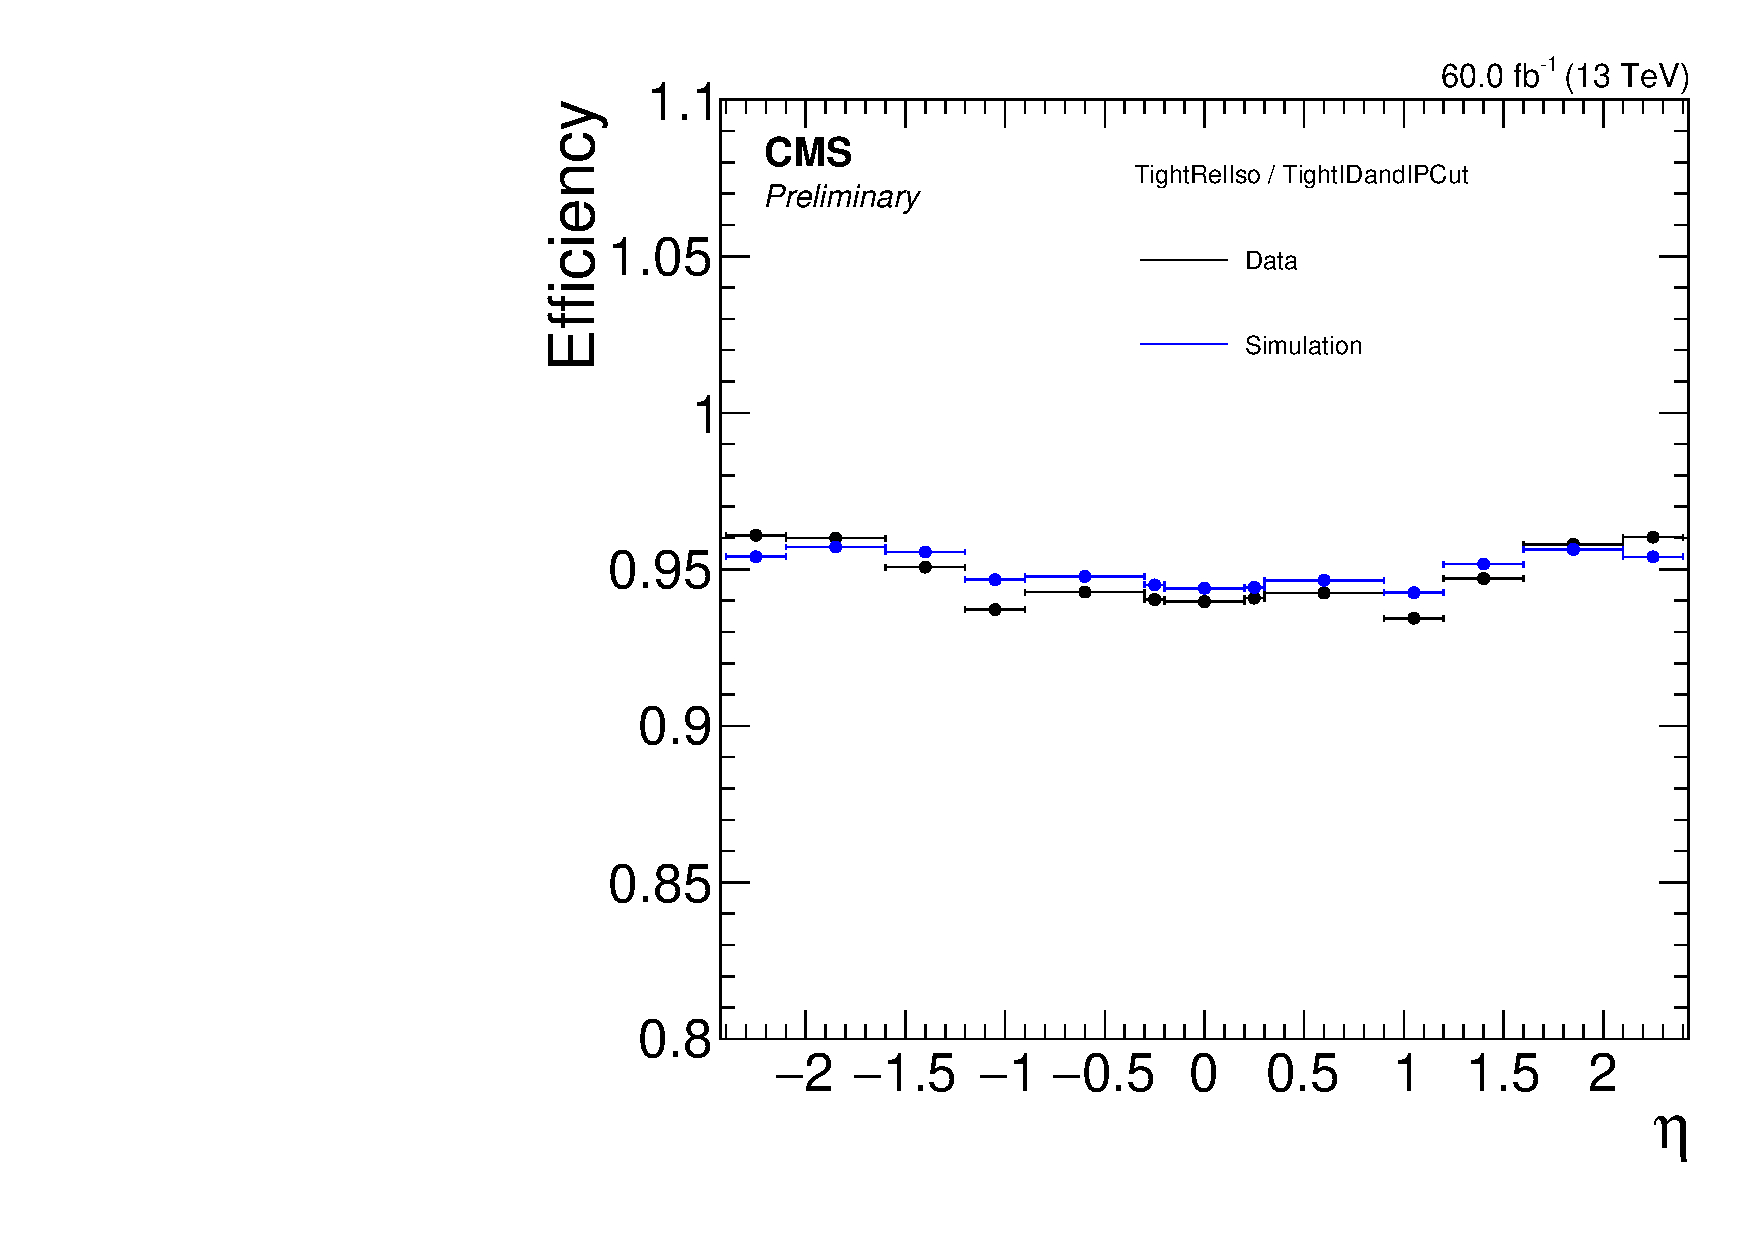
\includegraphics[width=0.45\textwidth]{figures/muonEtaEff.pdf}
        \hspace{0.01\textwidth}
        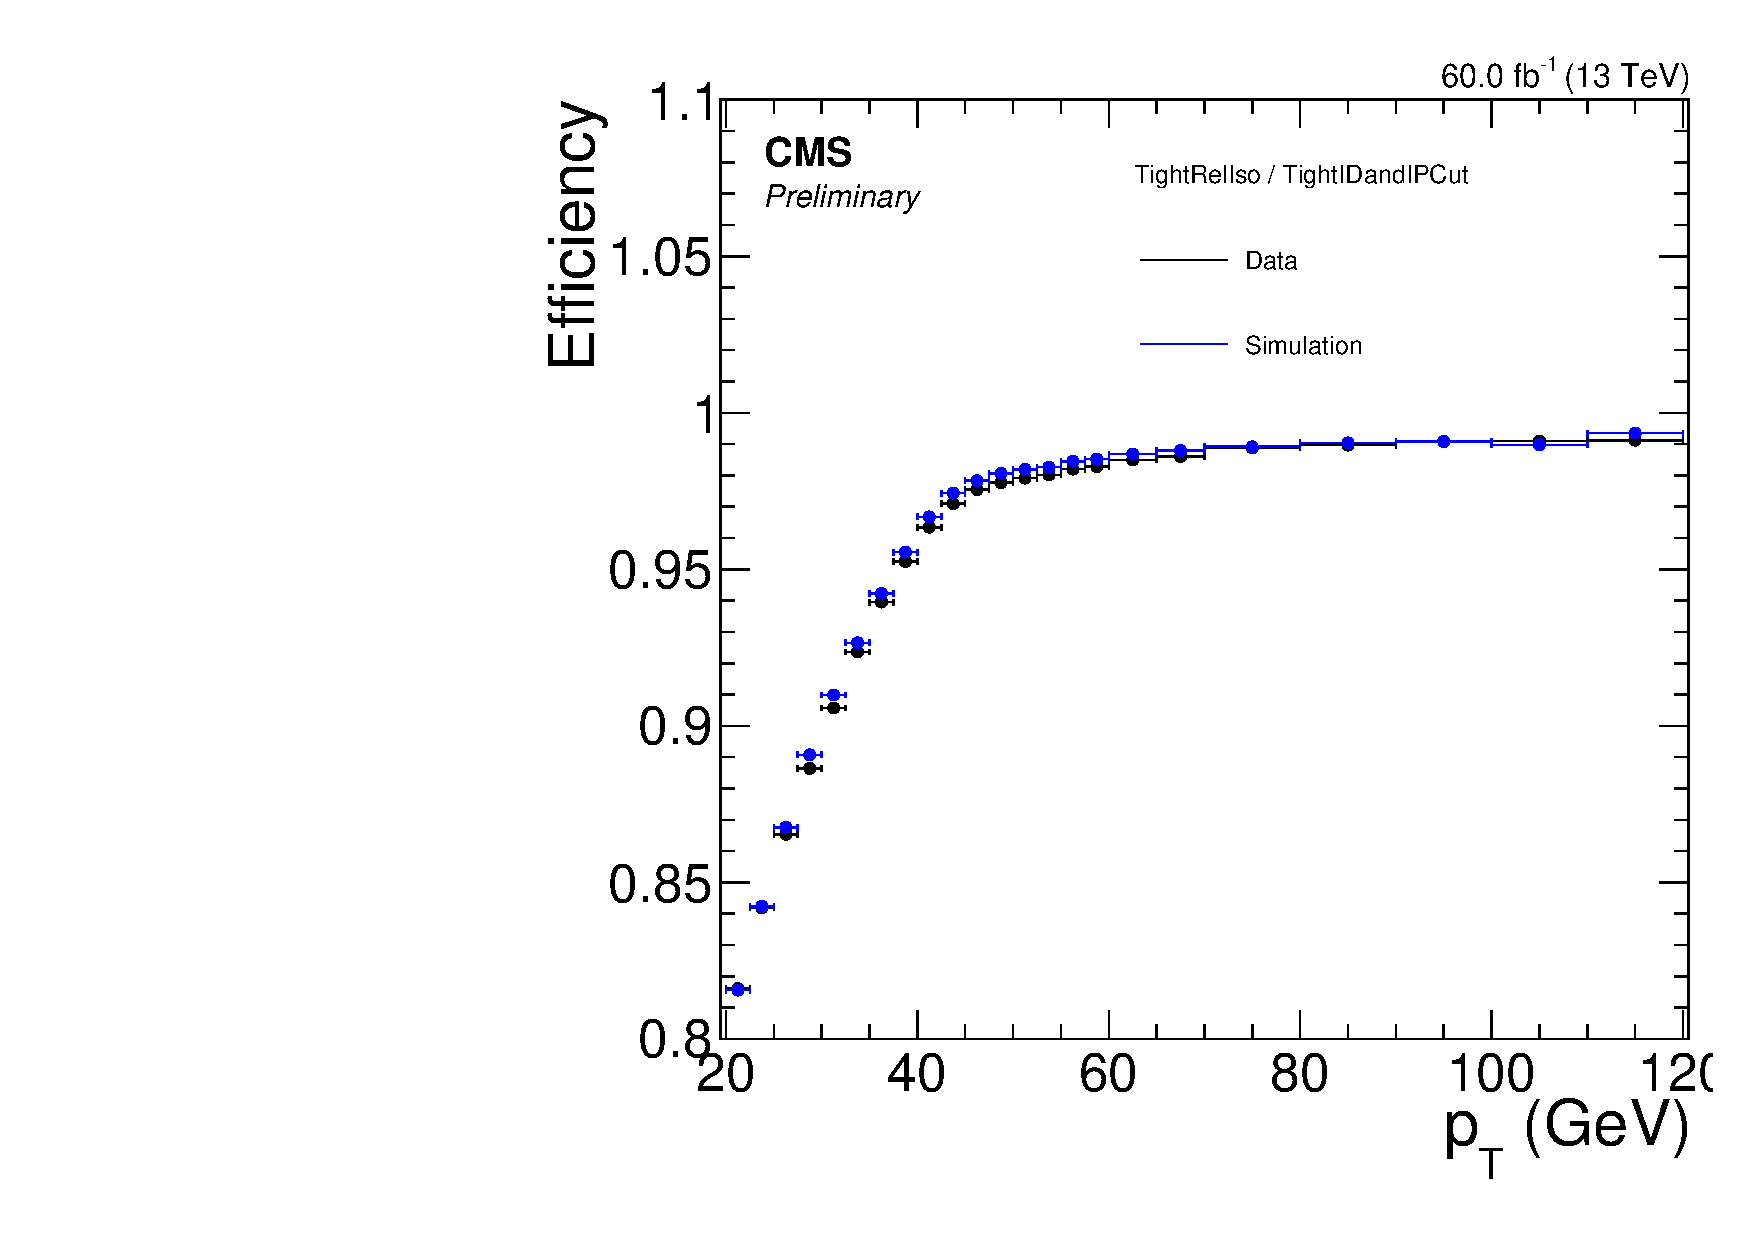
\includegraphics[width=0.45\textwidth]{figures/muonPtEff.pdf}
	\caption[Muon ID and Isolation Efficiencies]{Muon ID and Isolation efficiencies calculated using tag-and-probe methods as a function of $p_t$ (left) and $eta$ (right) for data and simulation. The ID and Isolation scale factors applied to simulated tagging muons are calculated using the ratio of the data and MC efficiencies within 2-dimensional $\eta$ and $p_t$ bins.}
        \label{fig:muIdIsoEff}
\end{figure}

\begin{figure}[htbp]
	\centering
	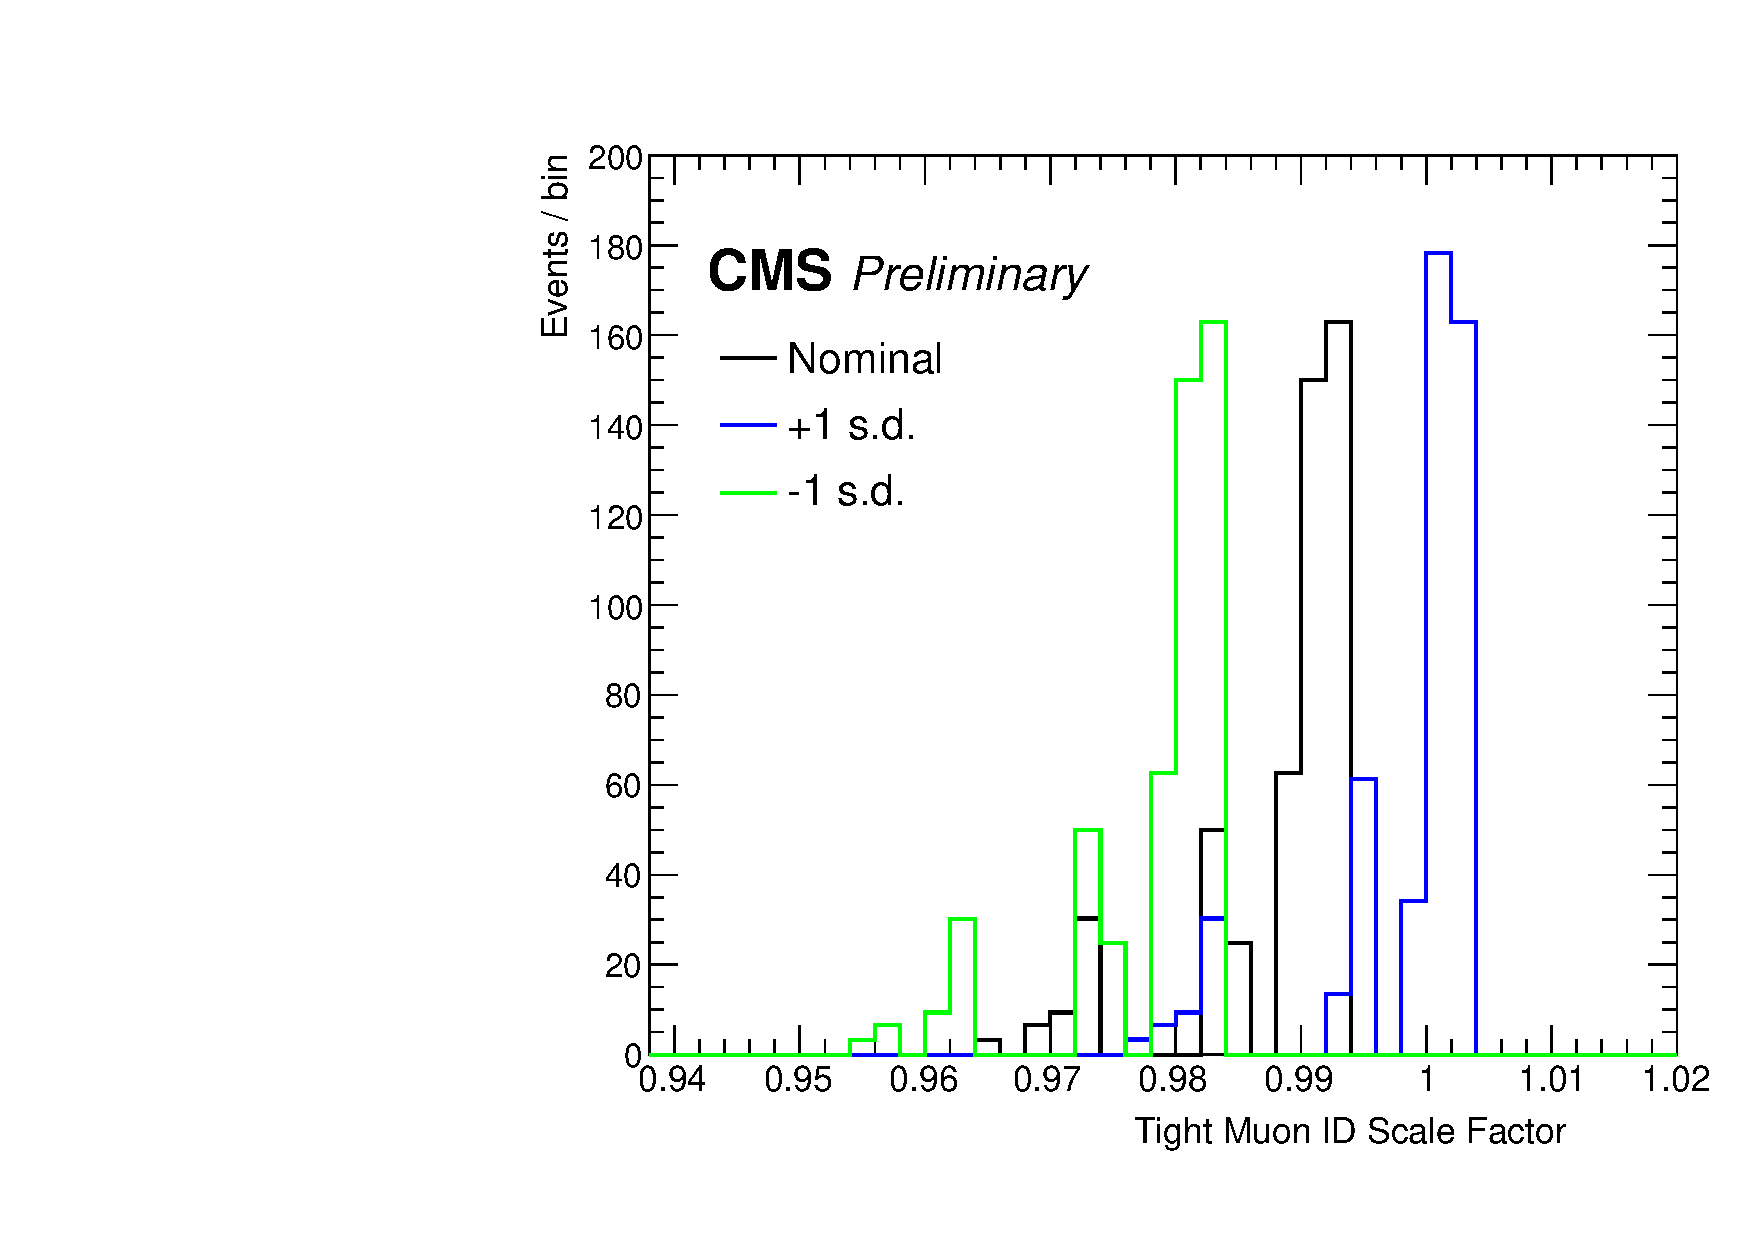
\includegraphics[width=0.45\textwidth]{figures/idSF.pdf}
        \hspace{0.01\textwidth}
        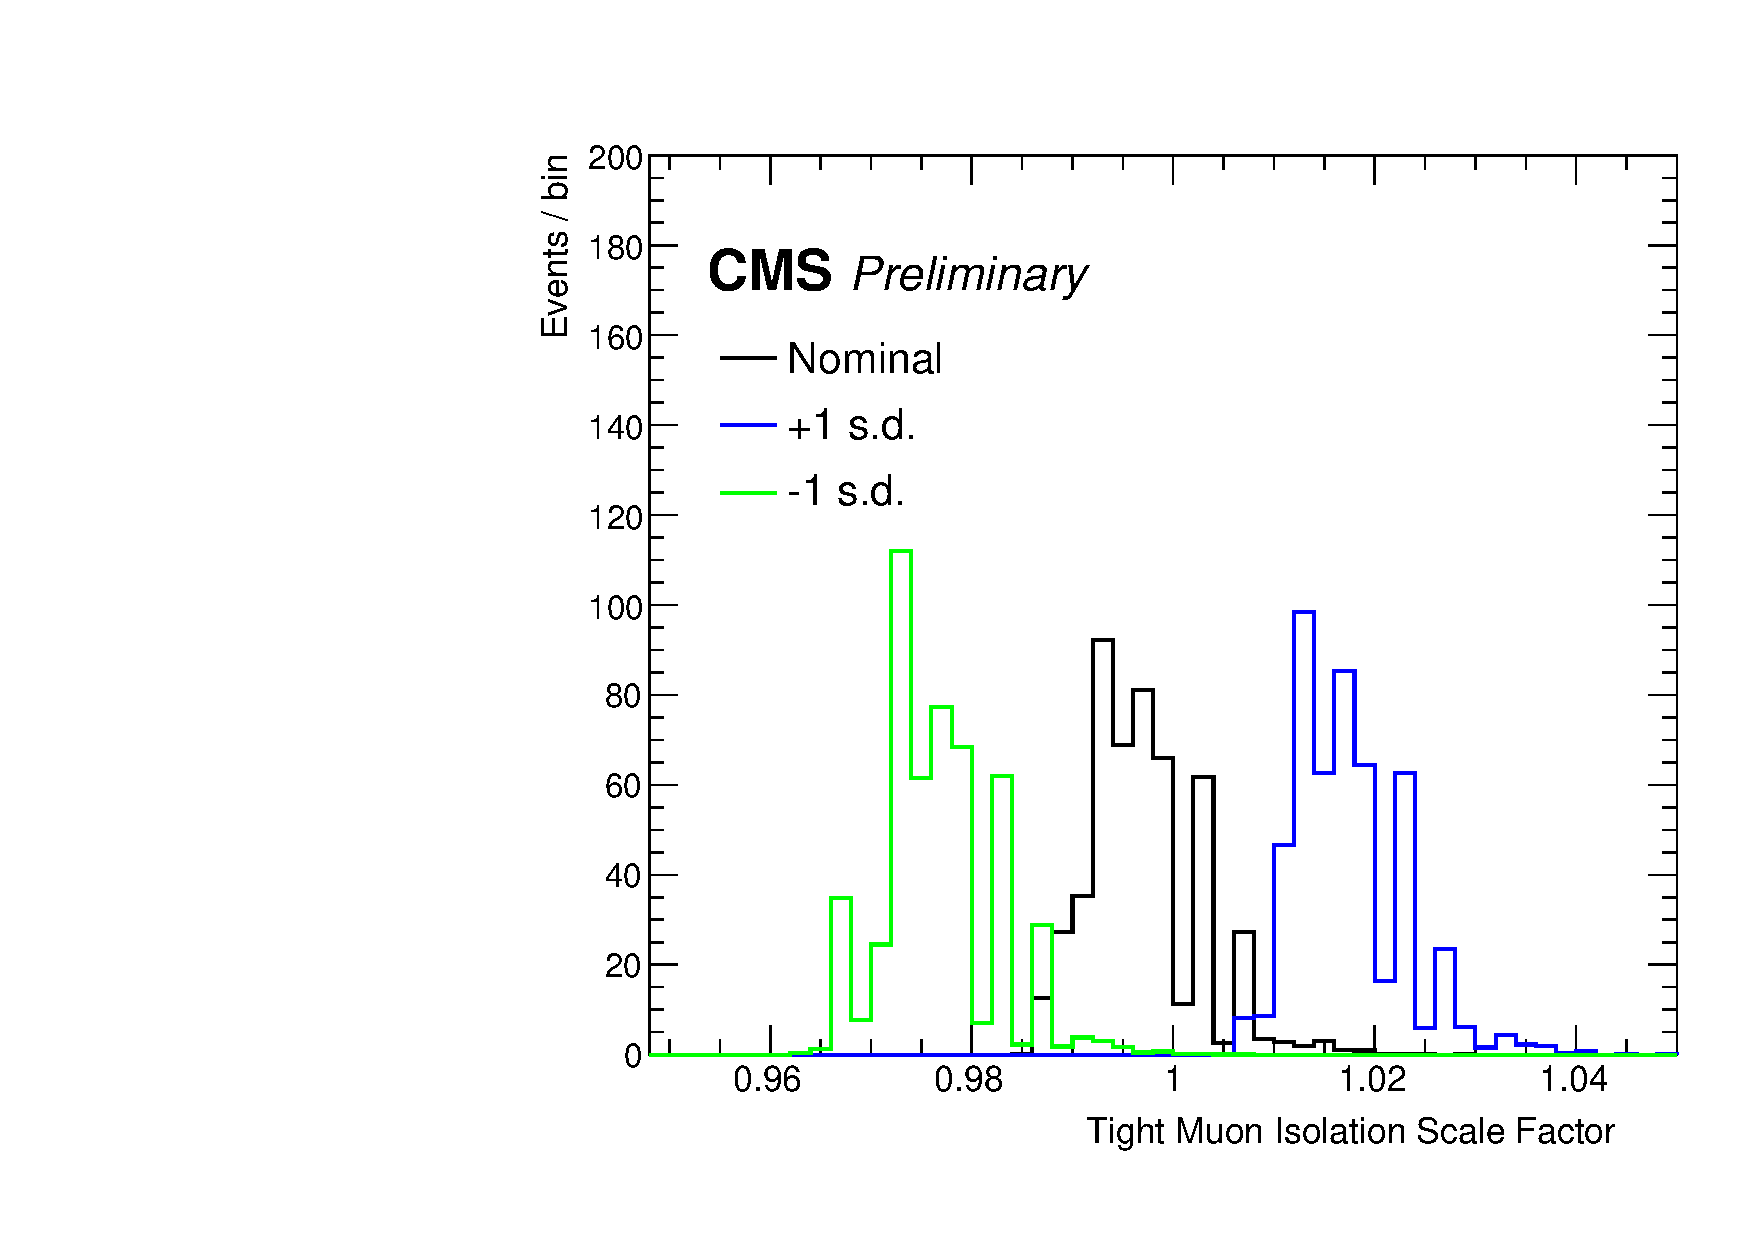
\includegraphics[width=0.45\textwidth]{figures/isoSF.pdf}
	\caption[Muon ID and Isolation Scale Factors]{The Muon ID and Isolation scale factors applied to the simulated DY events, calculated using the $\eta$ and $p_t$ of the tagging muon.}
        \label{fig:muIdIsoSFs}
\end{figure}

The efficiency of the isolated muon triggers used in this search are corrected using similar tag-and-probe techniques as the identification efficiency. 
By selecting events with high-quality tagging muons which pass the trigger requirements and probe muons with reduced identification requirements, the rate of muons with particular $\eta$, $\pt$, and isolation passing the trigger can be compared in data and MC.

All MC events are then re-weighted based on the relative rate of their tagging muons passing the trigger in data and MC, and a systematic uncertainty in this trigger efficiency is applied by changing the trigger efficiency by one standard deviation.
The measured trigger efficiencies, as well as the resulting weights and their up- and down-variations, are presented in \Cref{fig:muTrigSFs}.
To ensure that this efficiency is calculated for the correct muon, all tagging muons selected are required to pass the isolated muon trigger used in this search.

\begin{figure}[htbp]
	\centering
	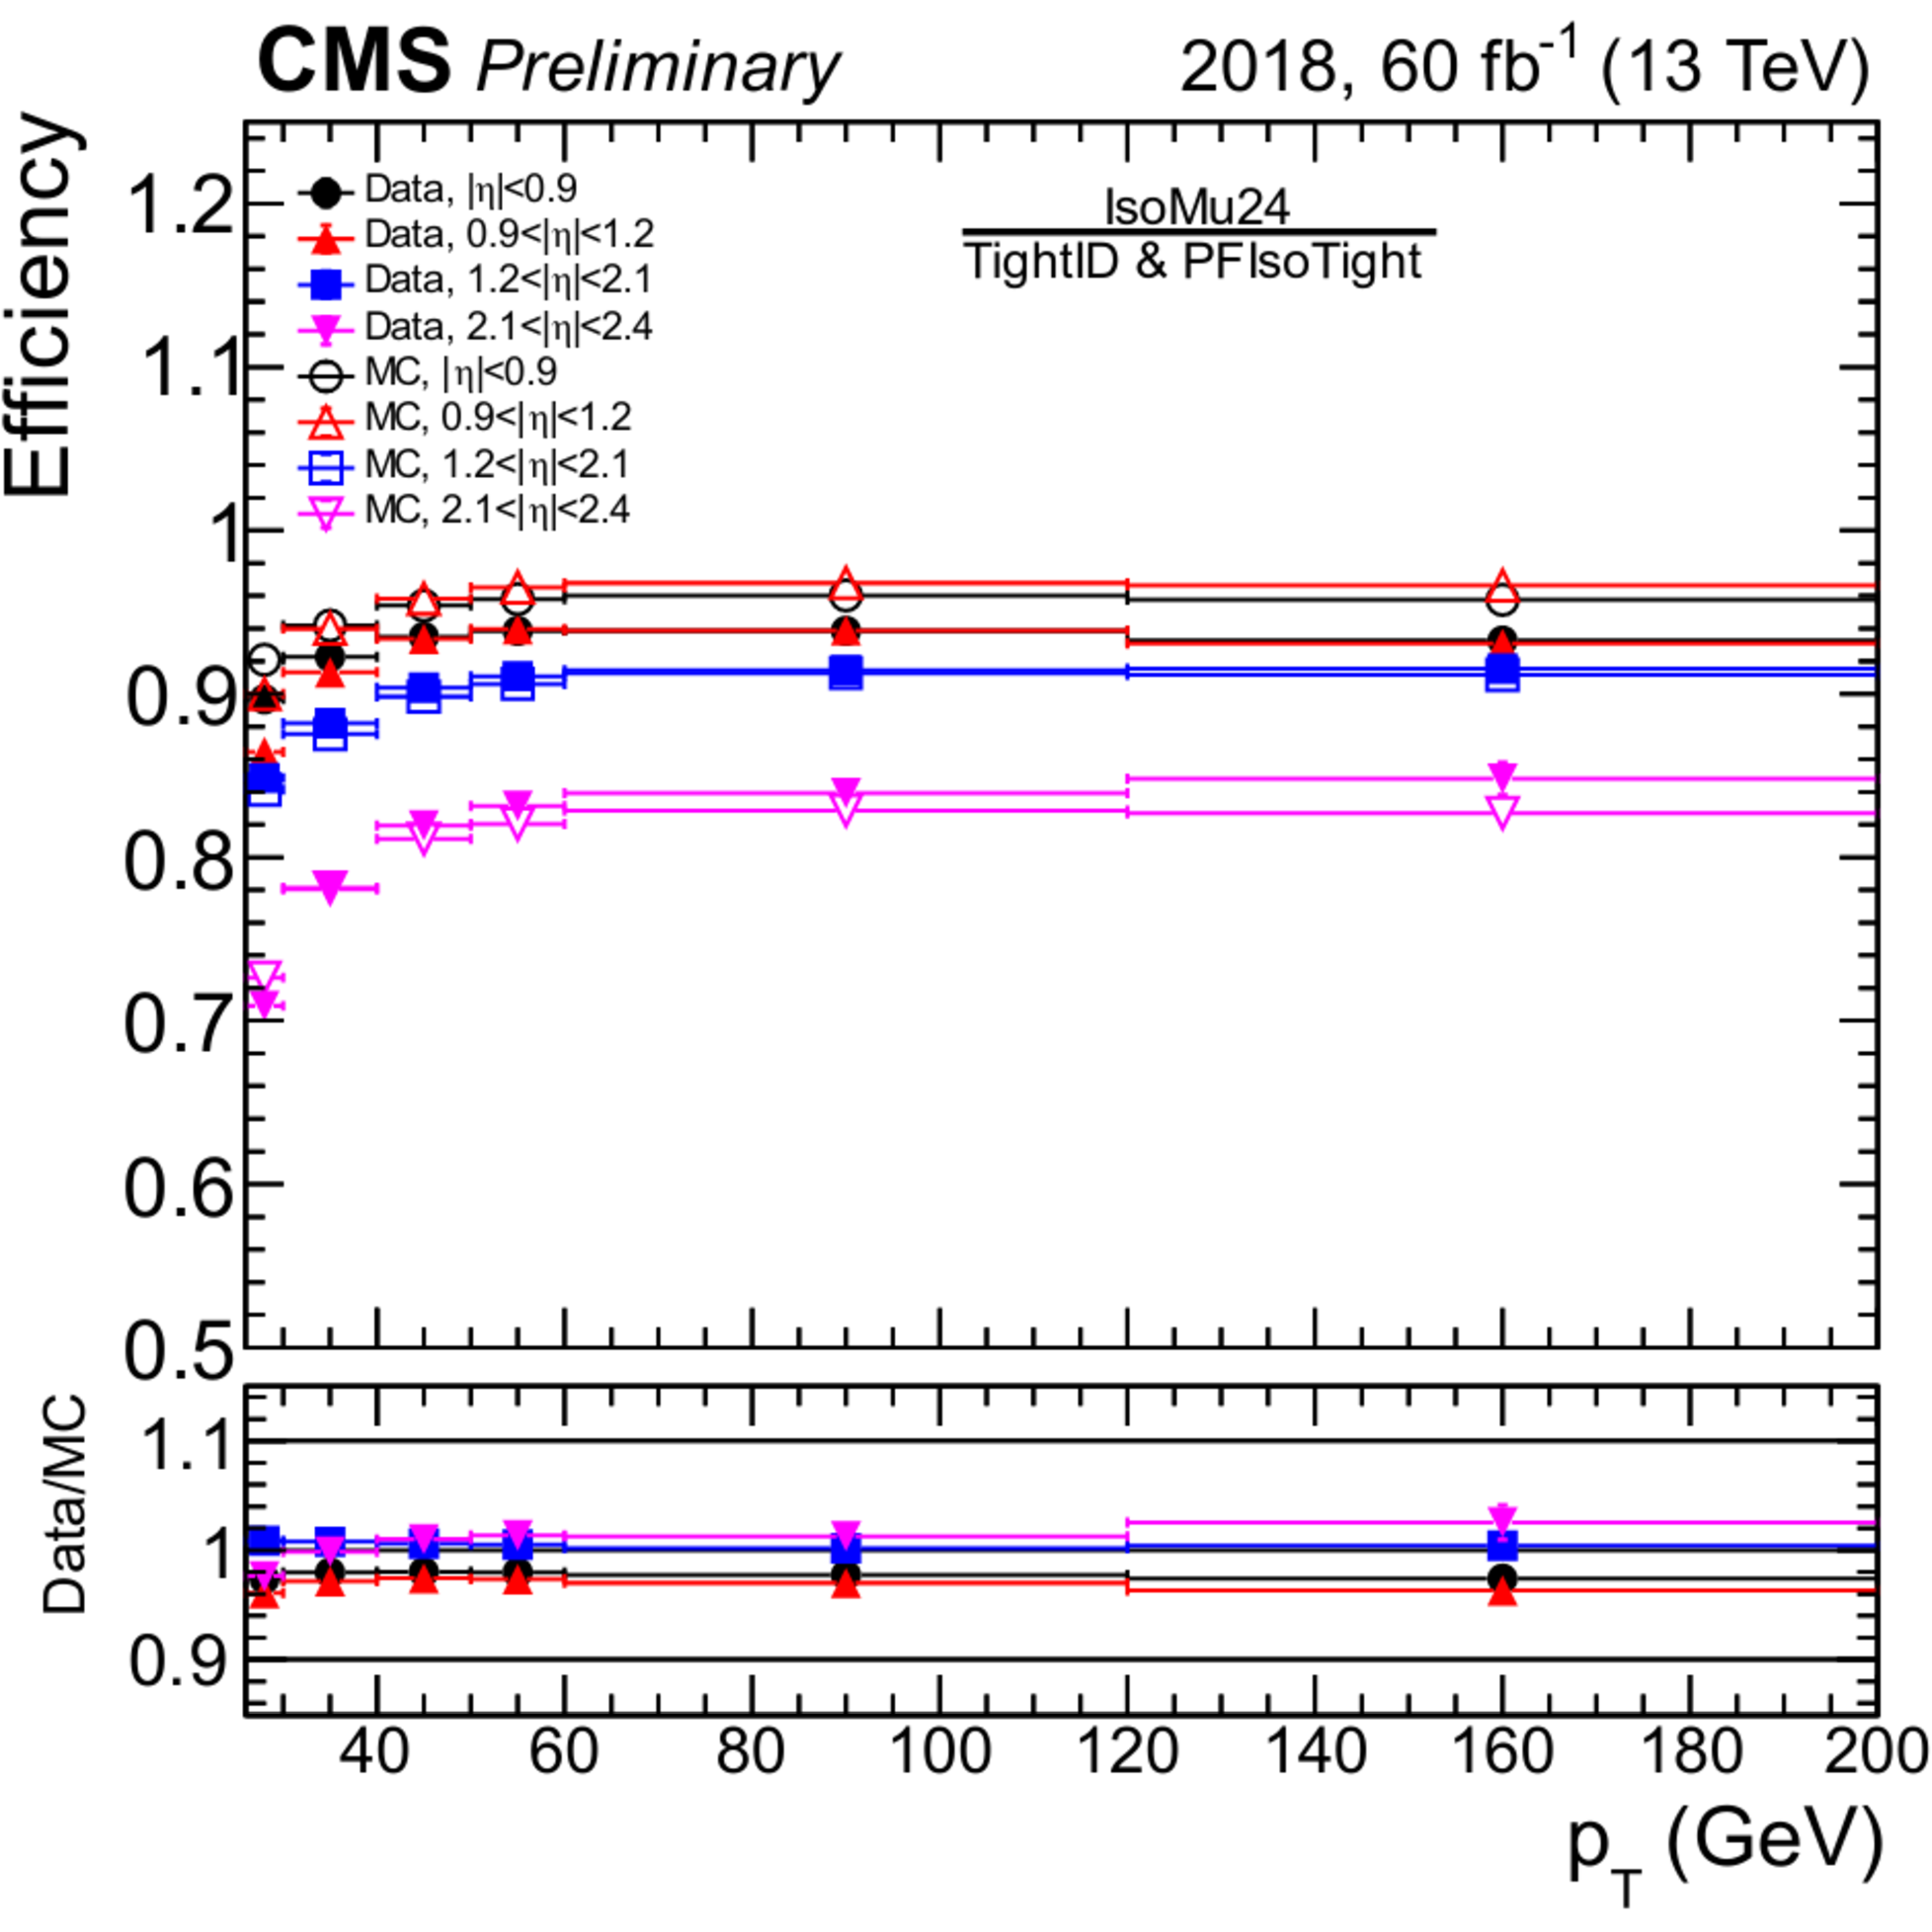
\includegraphics[width=0.5\textwidth]{figures/muTrigEff_2018.pdf}
        \hspace{0.01\textwidth}
        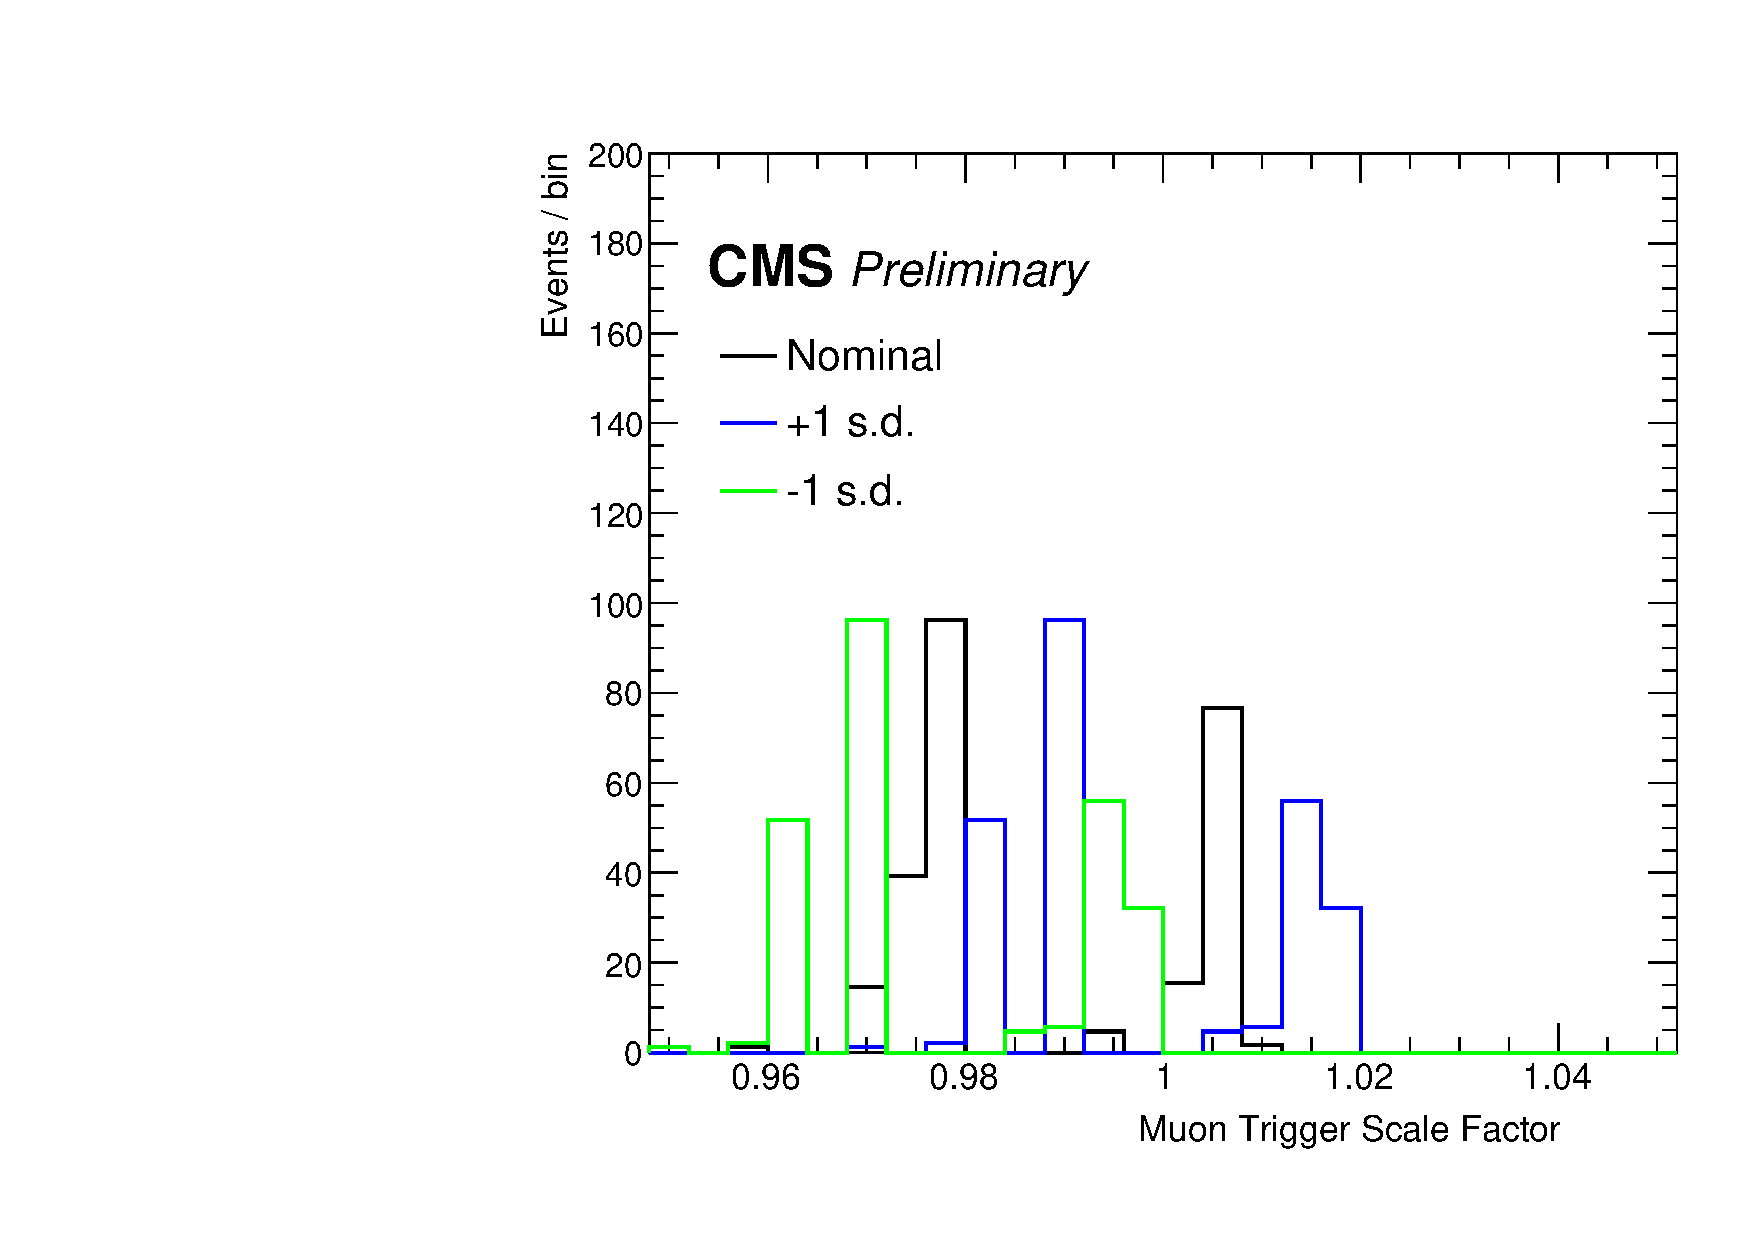
\includegraphics[width=0.45\textwidth]{figures/trigSF.pdf}
	\caption[Muon Trigger Scale Factors and Weights]{The isolation muon trigger scale factors as a function of muon $\eta$ and $\phi$ (left) and resulting weight (right) for DY MC events. The bi-modal distributions in the event weight are produced from the differences in typical scale factors between tagging muons in the barrel and endcap regions.}
        \label{fig:muTrigSFs}
\end{figure}

\subsection{Muon Energy Scale Corrections}
While this analysis does not strongly depend on the precision of the tagging muon kinematics, small differences that may be present between simulation and data in the tagging muon energy could cause shifts in the invariant mass distribution which would change the event acceptance rate.
To account for these potential differences, muon energy scale corrections are applied using the Rochester method~\cite{rochester_corr}.

The Rochester method is a data-driven correction to reconstructed muon energies as a function of $\eta$, $\phi$, and charge.
The correction is derived using a two-step approach which uses $Z/\gamma* \rightarrow \mu\mu$ events.
In the first step, DY events are generated for a perfectly aligned detector by smearing the generator level momentum using a function that replicates the experimental resolution as a function of $\eta$. 
Corrections for both data and MC are then derived by requiring that the average $1/p_t^\mu$ of muons from Z decays matches the perfectly-aligned MC.

In the second step, further corrections are derived for each $\eta-\phi$ bin so that the reconstructed Z mass is the same as the perfectly aligned detector. 
This step removes scatter in average Z mass which can result from the first step due to variations in muon efficiency between $\eta-\phi$ bins that are not perfectly modeled in MC. 
The muon energy scale corrections are applied to all tagging muons, and uncertainties in the resulting muon momentum are included as an overall systematic based on the change in signal efficiency produced when varying them by one standard deviation.

\subsection{HCAL Efficiencies}
\label{sec:HCALeff}
The response of the HCAL to muons is important in this study to reject events with large energy deposits as well as events where the selected probe did not reach the calorimeters.
In addition, the depth-by-depth information can be used to search for evidence of a change in muon energy within HE as a signature of a \dbrem.
In order to use this level of detail, the muon HCAL deposits in MC must be validated and corrected to match those seen in data.
This is done through study of muon deposits along the trajectory of selected tagging muons.

As the global muon associated with the tagging muon may have improved trajectory accuracy due to the inclusion of information from the muon systems, only the inner track matching the global muon is projected into HE to match the information available for selected probes in the final analysis.
The HCAL energy is then collected in each depth along the trajectory of the track, and the distributions of energy are compared in data and DY MC.

The energy distributions along tag-muon aligned tracks for the first and fourth HE depths are shown in \Cref{fig:unCorrHEDepths}.
As the depth increases, the thickness of the layers increases and deposits from pileup decrease, as nearby non-muon particles are absorbed by the calorimeter, improving the amplitude and resolution of the muon peak.
The simulated and data events were found to have peak energies near the same values but significant excesses of events with very low energy ($<$\SI{0.1}{\giga\eV}) were seen in data, while simulated events were seen to have higher rates of events with large HE energy deposits.

\begin{figure}[htbp]
	\centering
	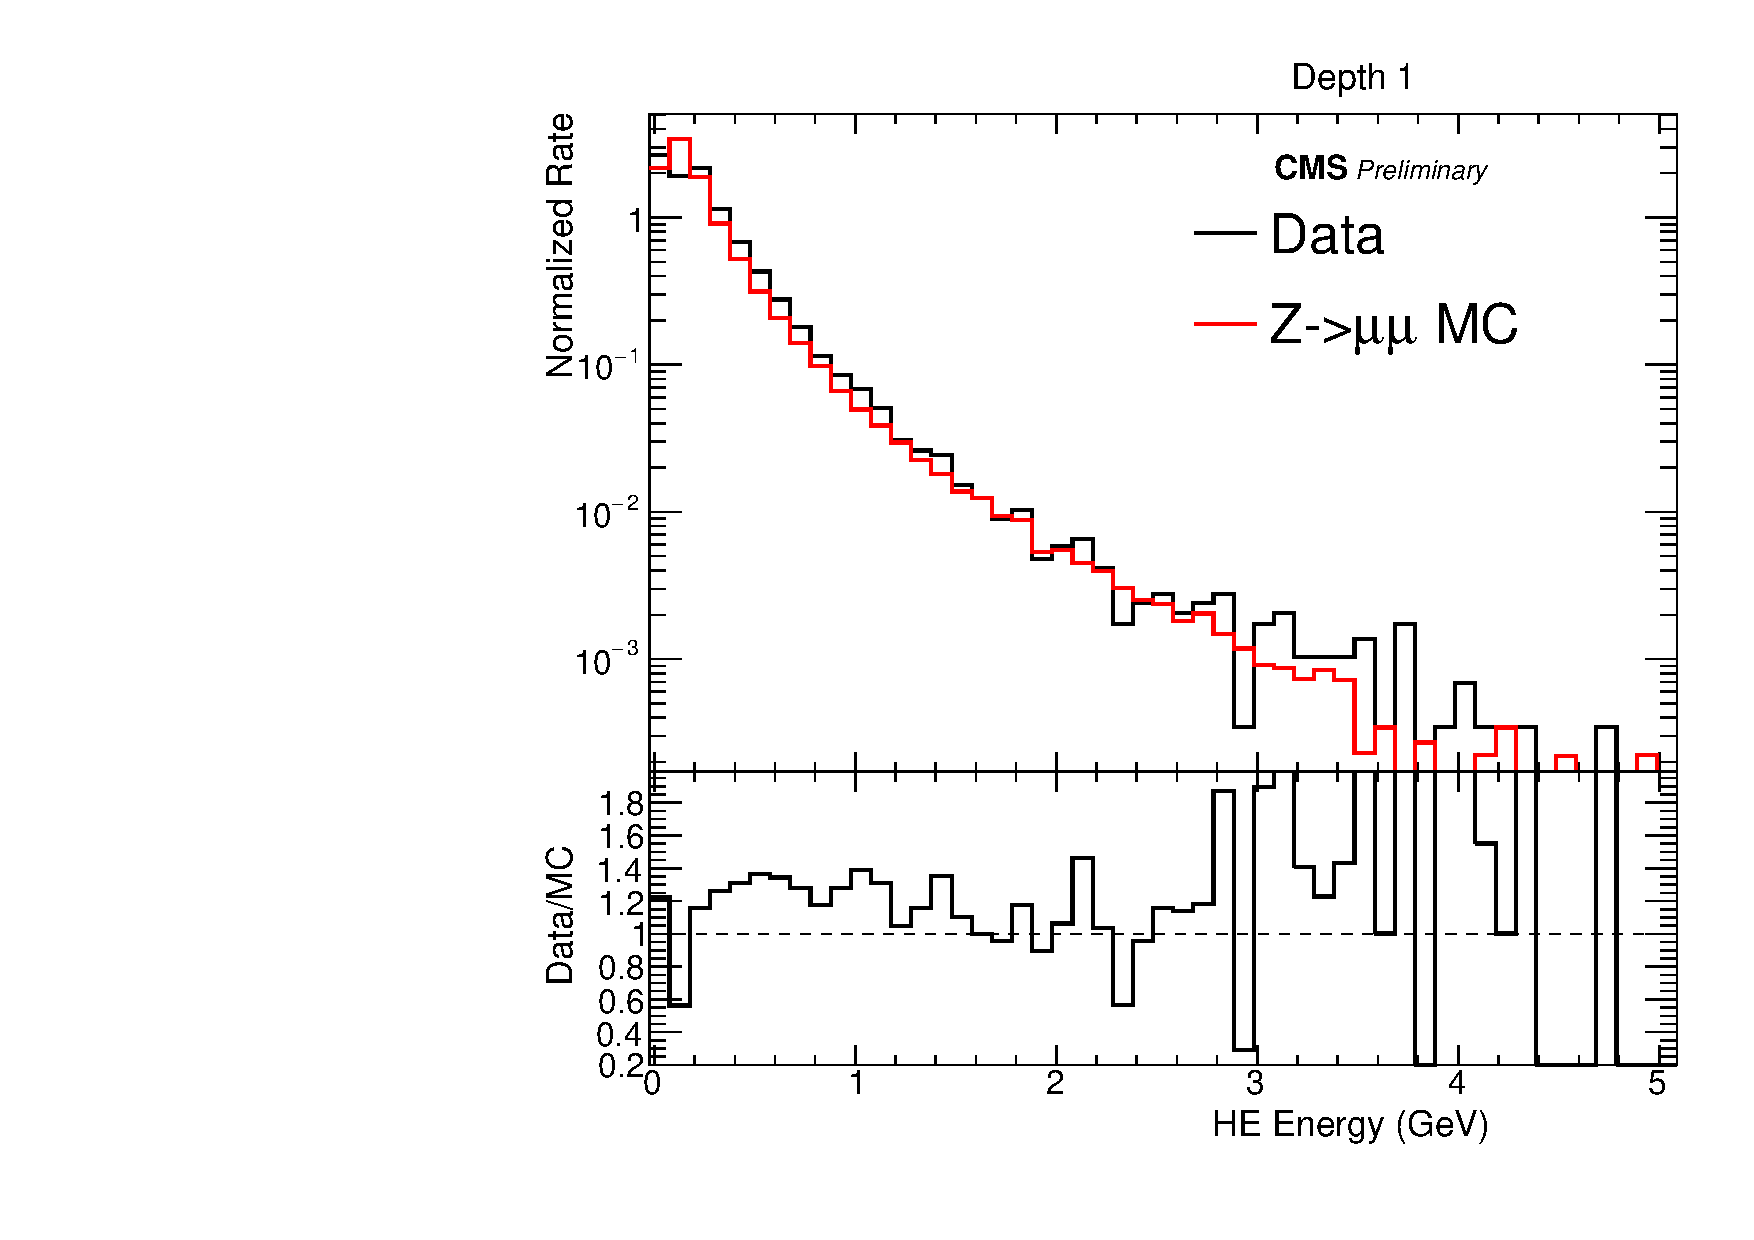
\includegraphics[width=0.45\textwidth]{figures/hcalAllE_depth0.pdf}
        \hspace{0.01\textwidth}
        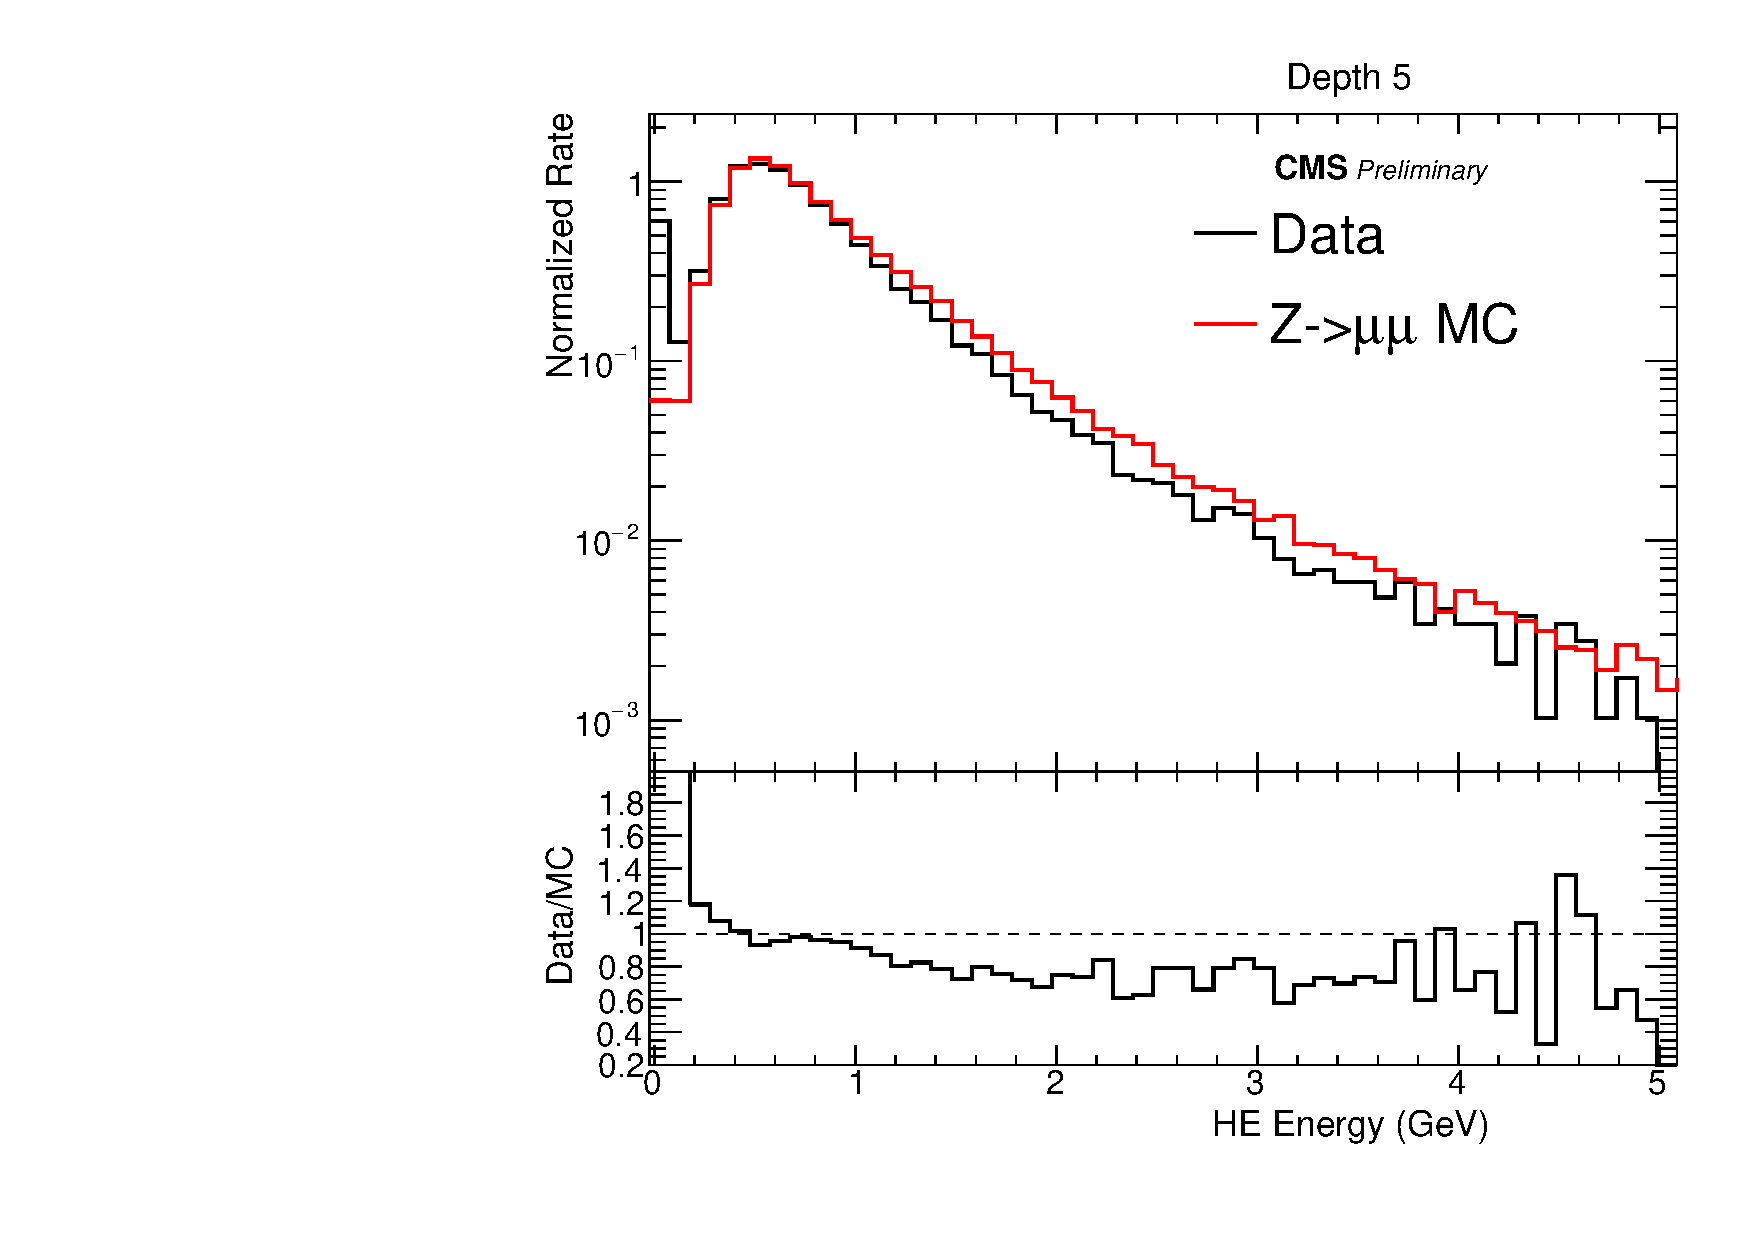
\includegraphics[width=0.45\textwidth]{figures/hcalAllE_depth4.pdf}
        \caption[HE Energy Deposits Along Tag-Aligned Muons]{The HE energy for two individual depths from cells aligned with tagging muons. Significant excess is seen in data events with very low HE energy and MC events with large energy.}
        \label{fig:unCorrHEDepths}
\end{figure}

To study these events, the number of depths with less than \SI{0.1}{\giga\eV}, referred to as 'missing hits' (\Cref{fig:missingHits}), was measured for each event and a sub-sample of events with multiple missing hits was created. 
Events with many missing hits were found to correspond to probe trajectories that align with the edges of HE cells (\Cref{fig:cellEdges}), and are likely caused by a combination of effects from differences in light collection efficiency with particle position that are not replicated in simulation, gaps between cells causing small regions of missing coverage, and misalignment between the CMS tracker and HCAL in reconstruction.

\begin{figure}[htbp]
	\centering
	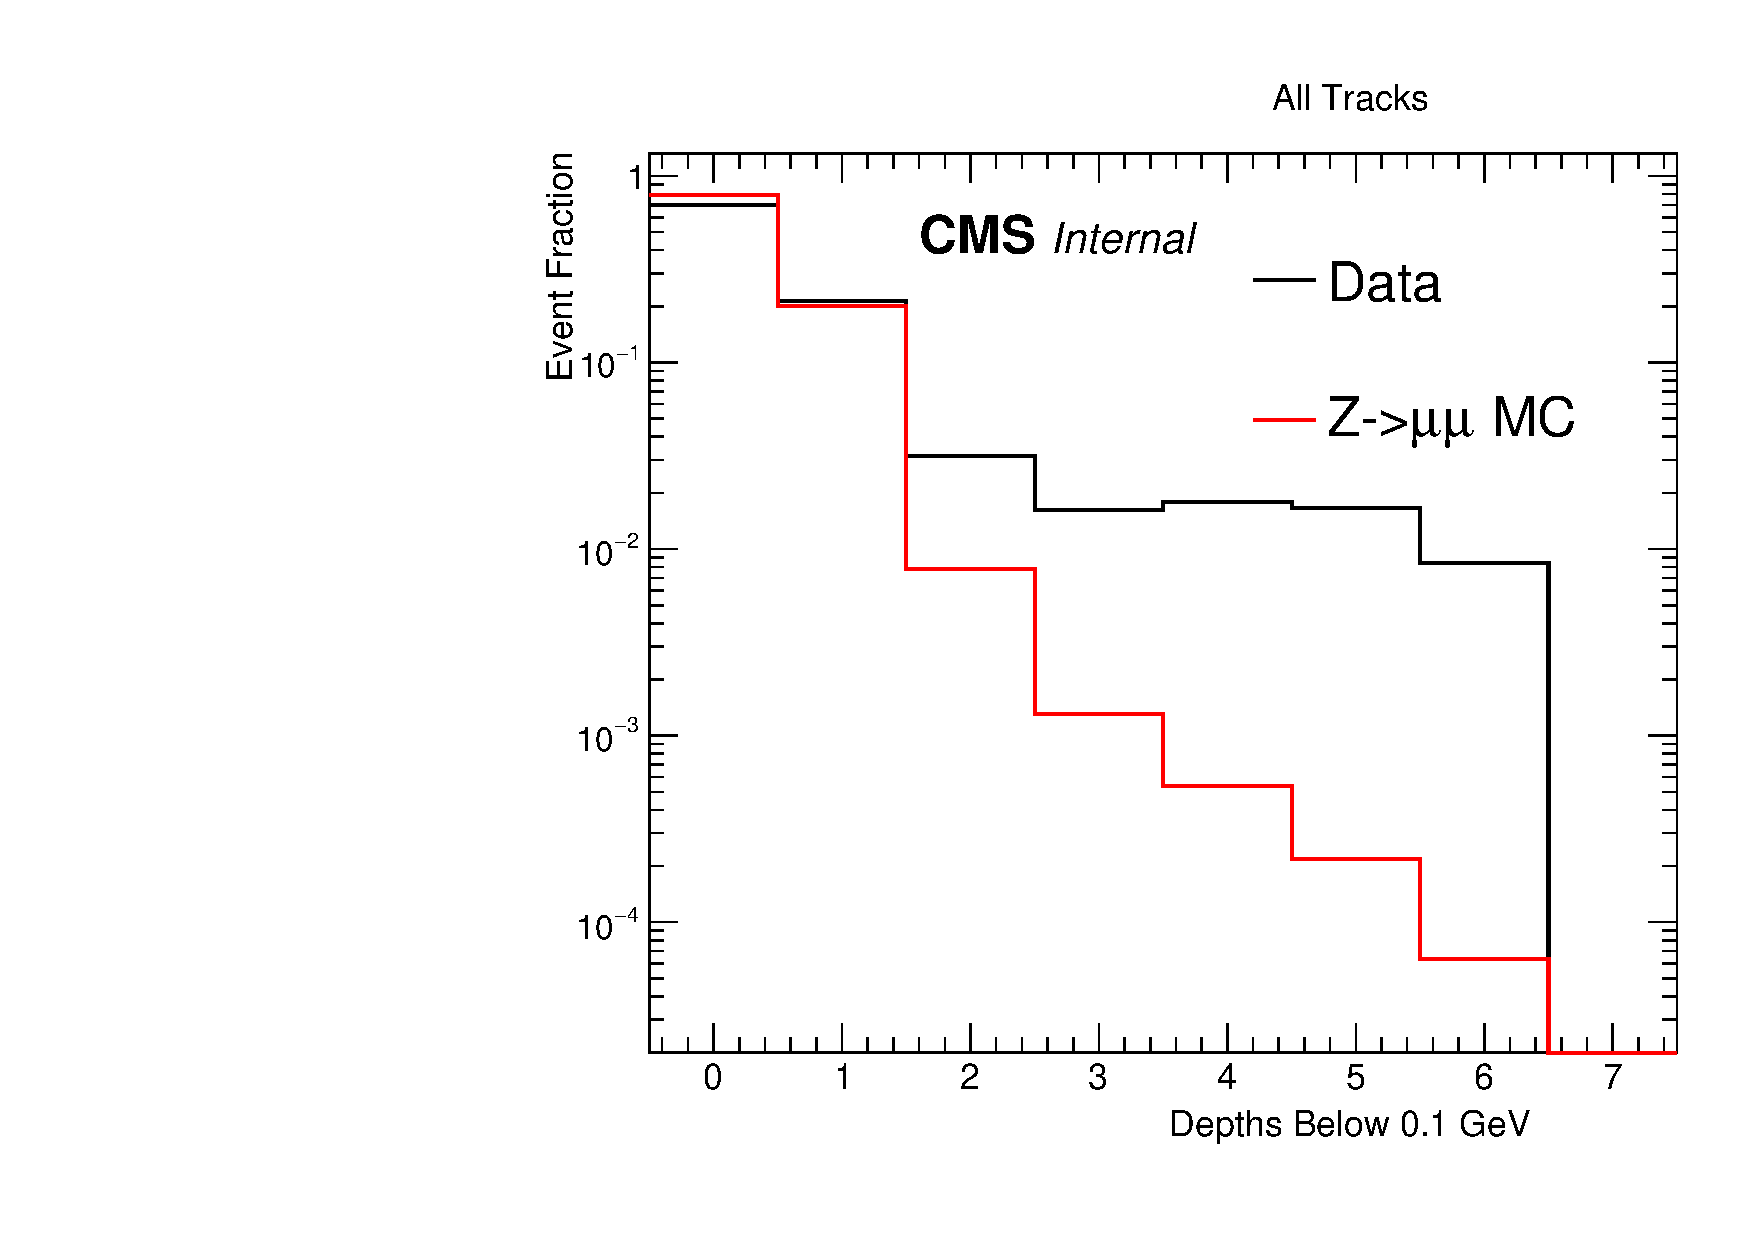
\includegraphics[width=0.45\textwidth]{figures/hcalAllMissingHits.pdf}
        \hspace{0.01\textwidth}
        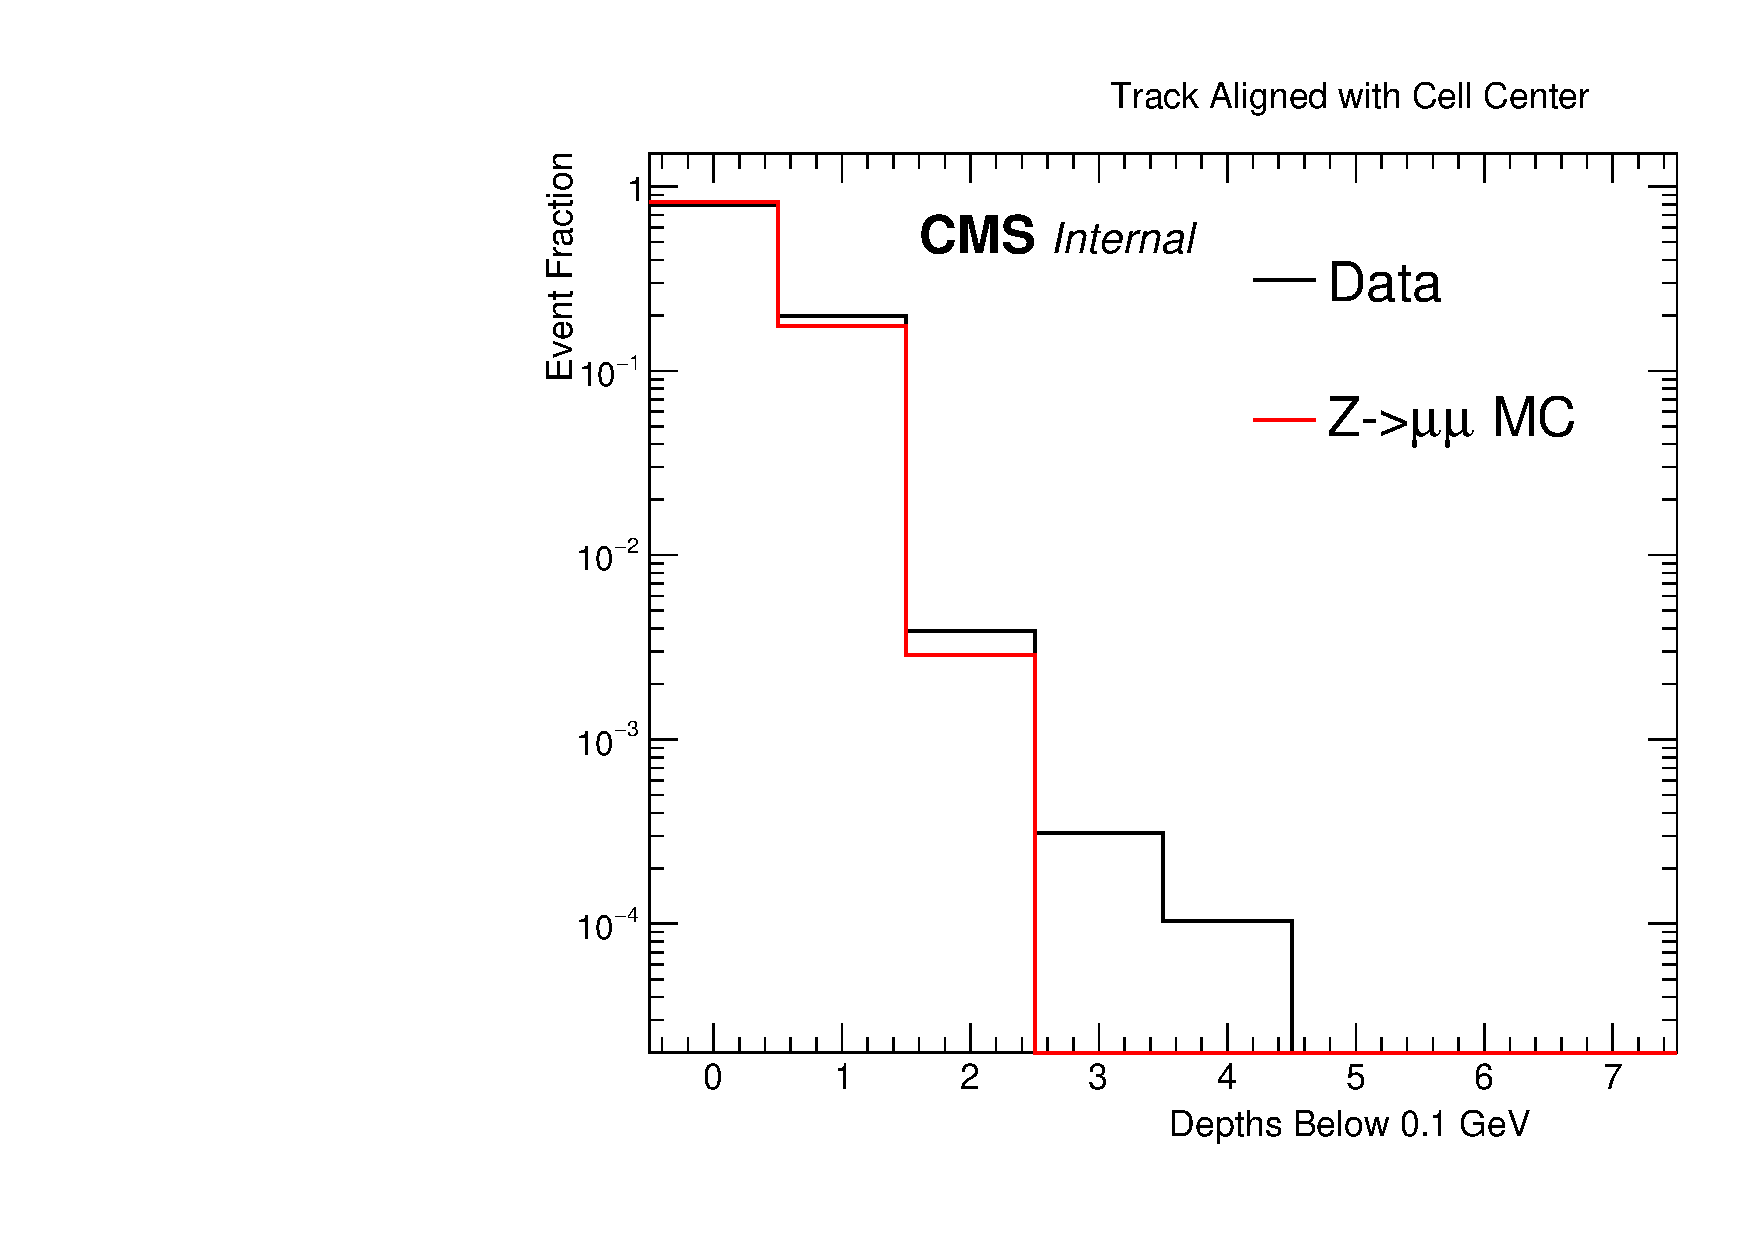
\includegraphics[width=0.45\textwidth]{figures/hcalMissingHits.pdf}
        \caption[Missing muon hits in HE]{The number of HE depths along tagging muon trajectories below \SI{0.1}{\giga\eV} for all selected muons (left) and for those not near HE cell edges (right). Significant excess in events with many missing hits is seen in data events with tracks near cell edges, and the non-exponential shape of the data events indicates that there is some systematic effect producing these missing hits.}
        \label{fig:missingHits}
\end{figure}

\begin{figure}[htbp]
	\centering
	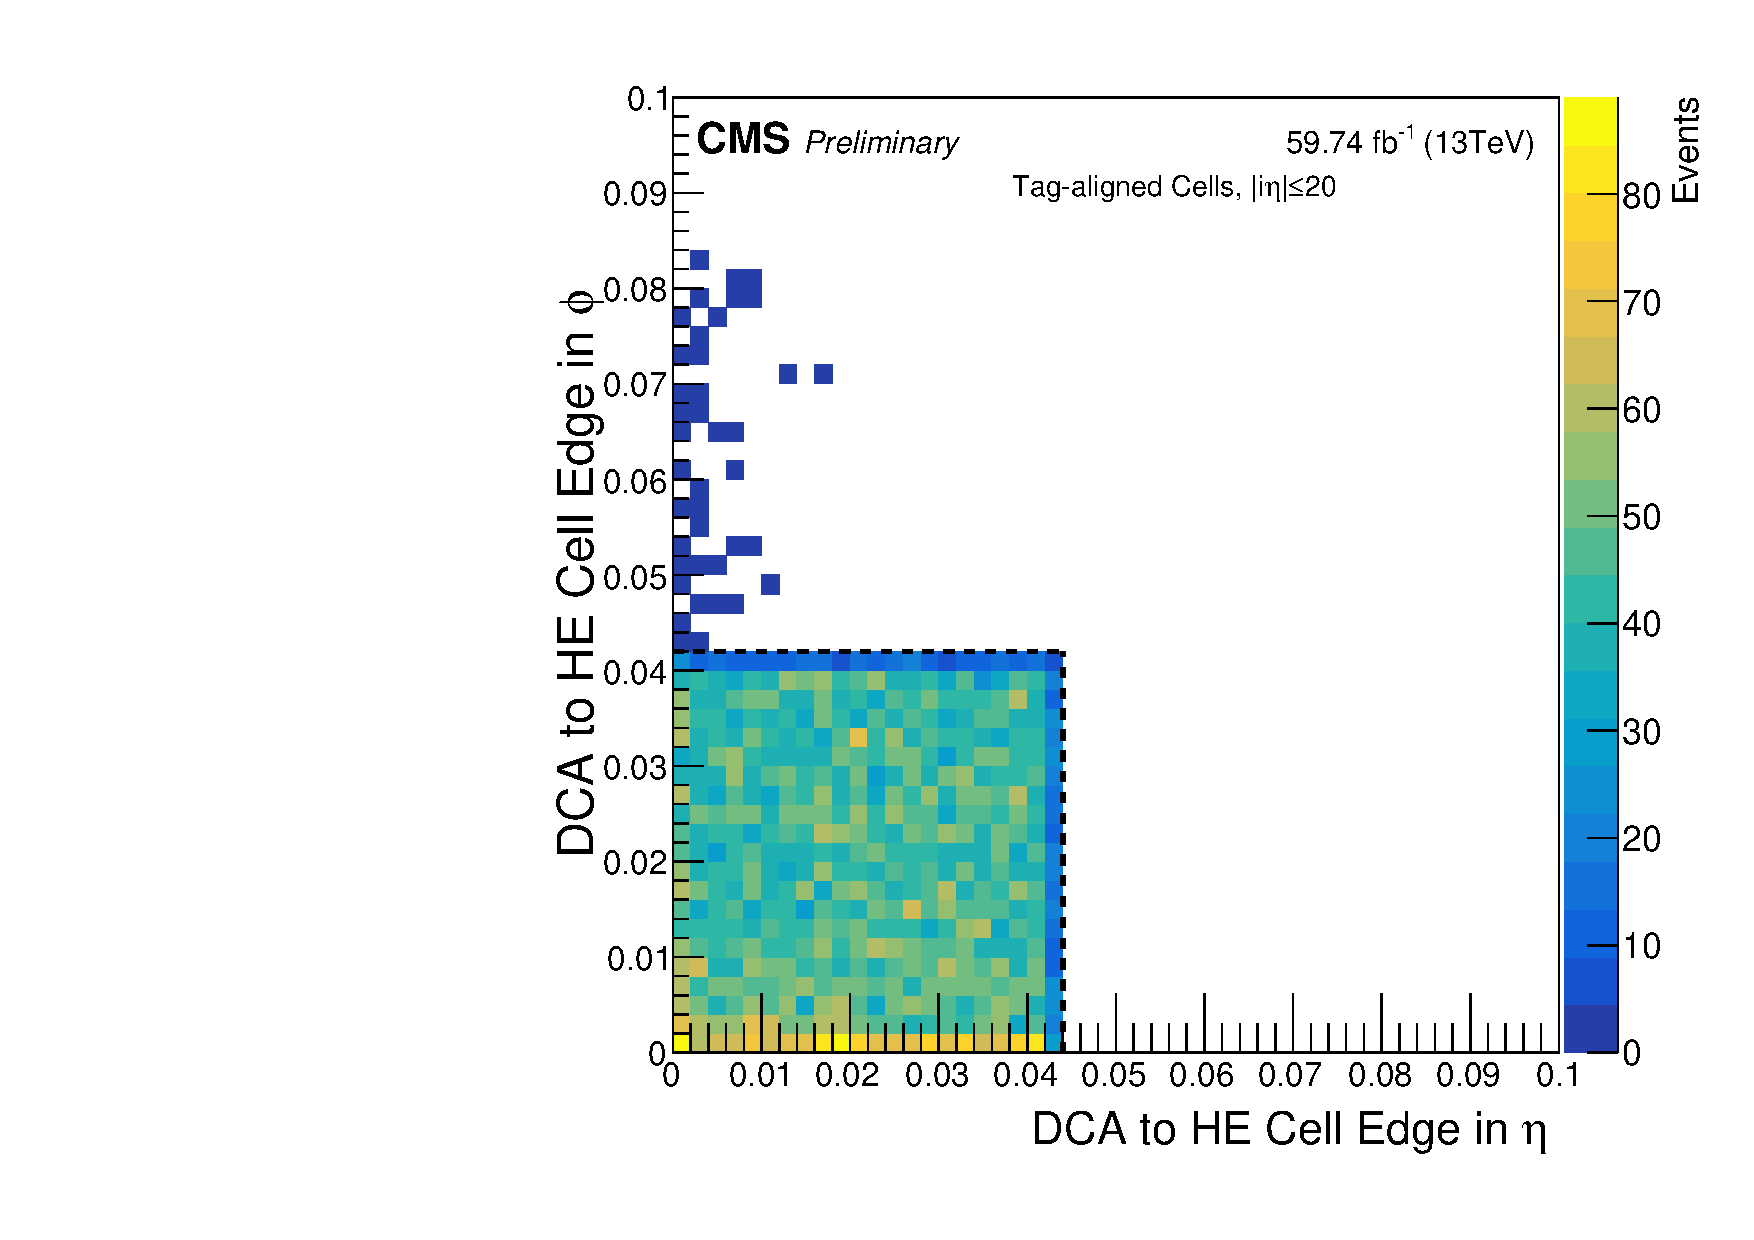
\includegraphics[width=0.45\textwidth]{figures/HEEdgeDistance_all_smallCell.pdf}
        \hspace{0.01\textwidth}
        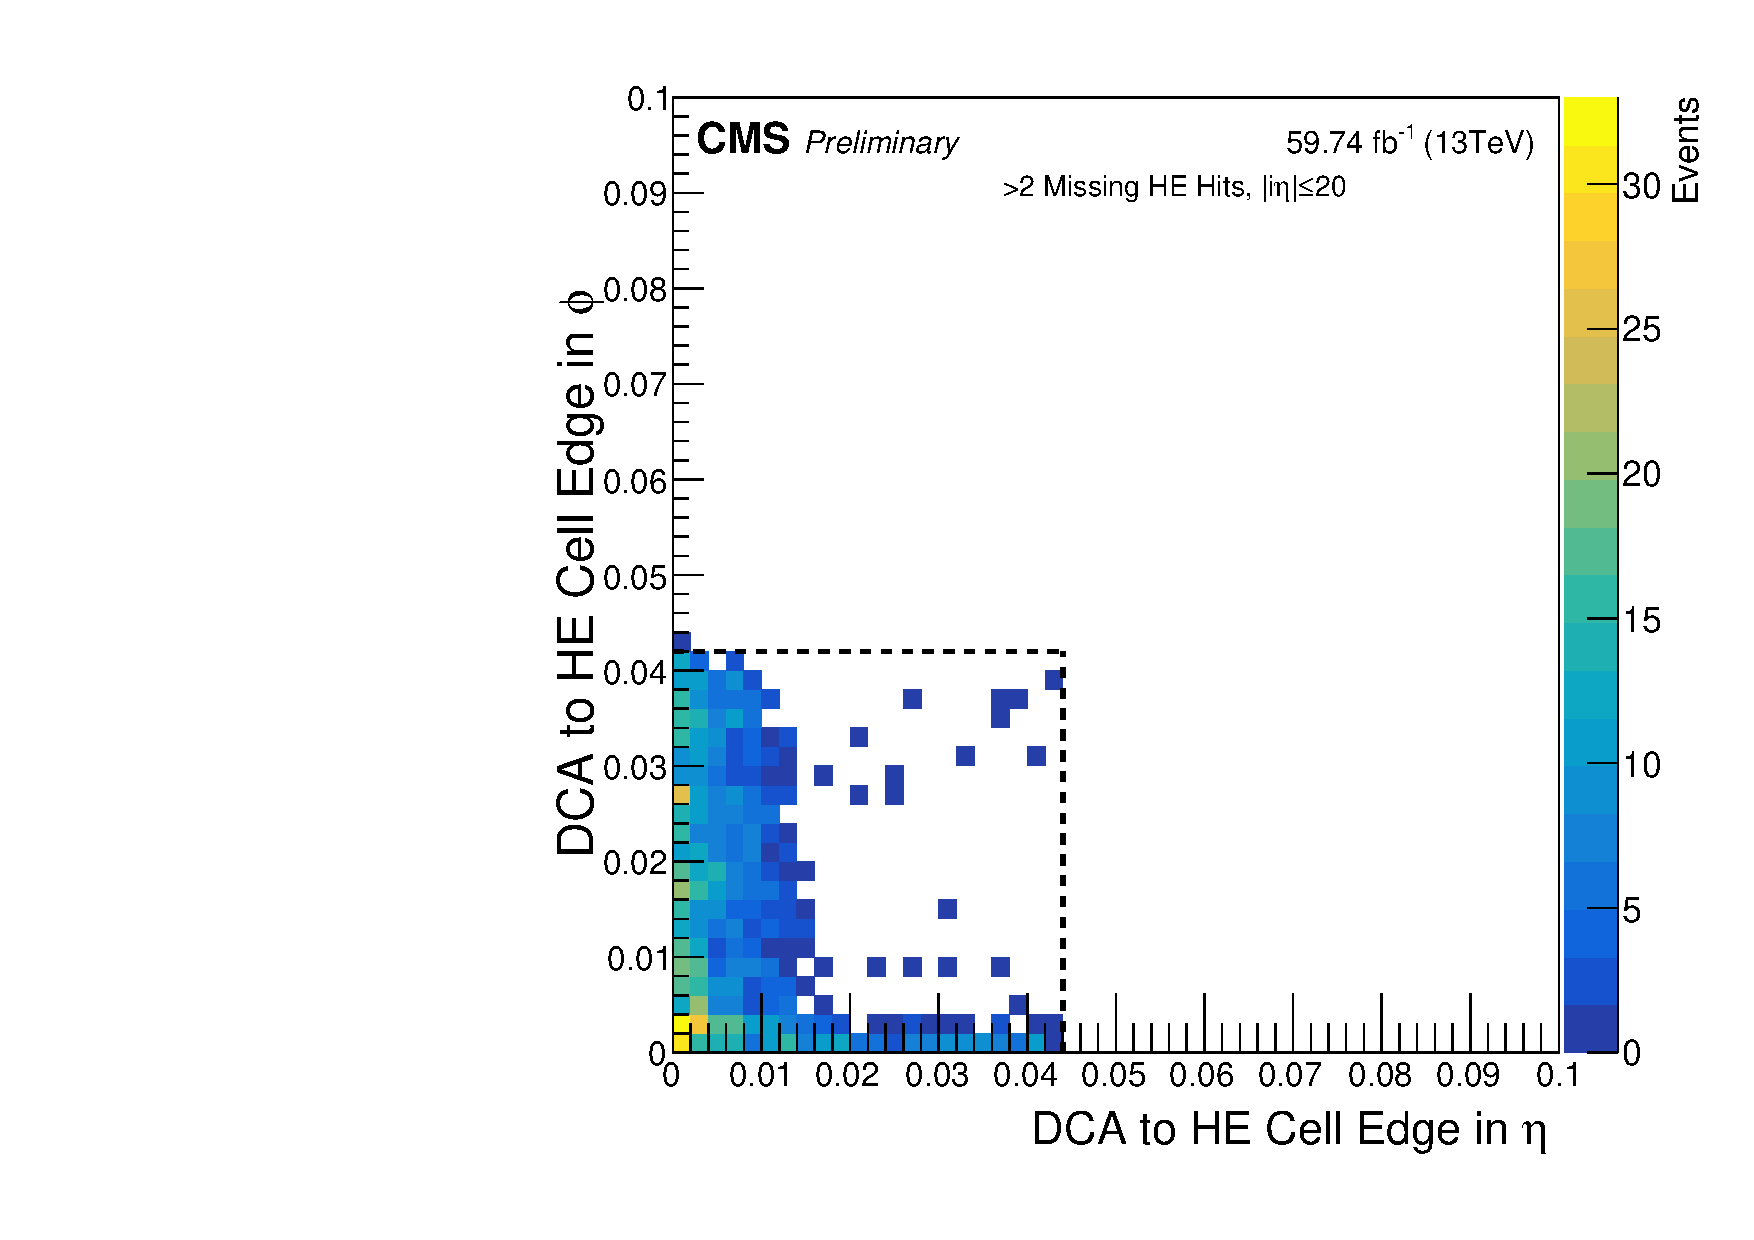
\includegraphics[width=0.45\textwidth]{figures/HEEdgeDistance_multMissing_smallCell.pdf}
	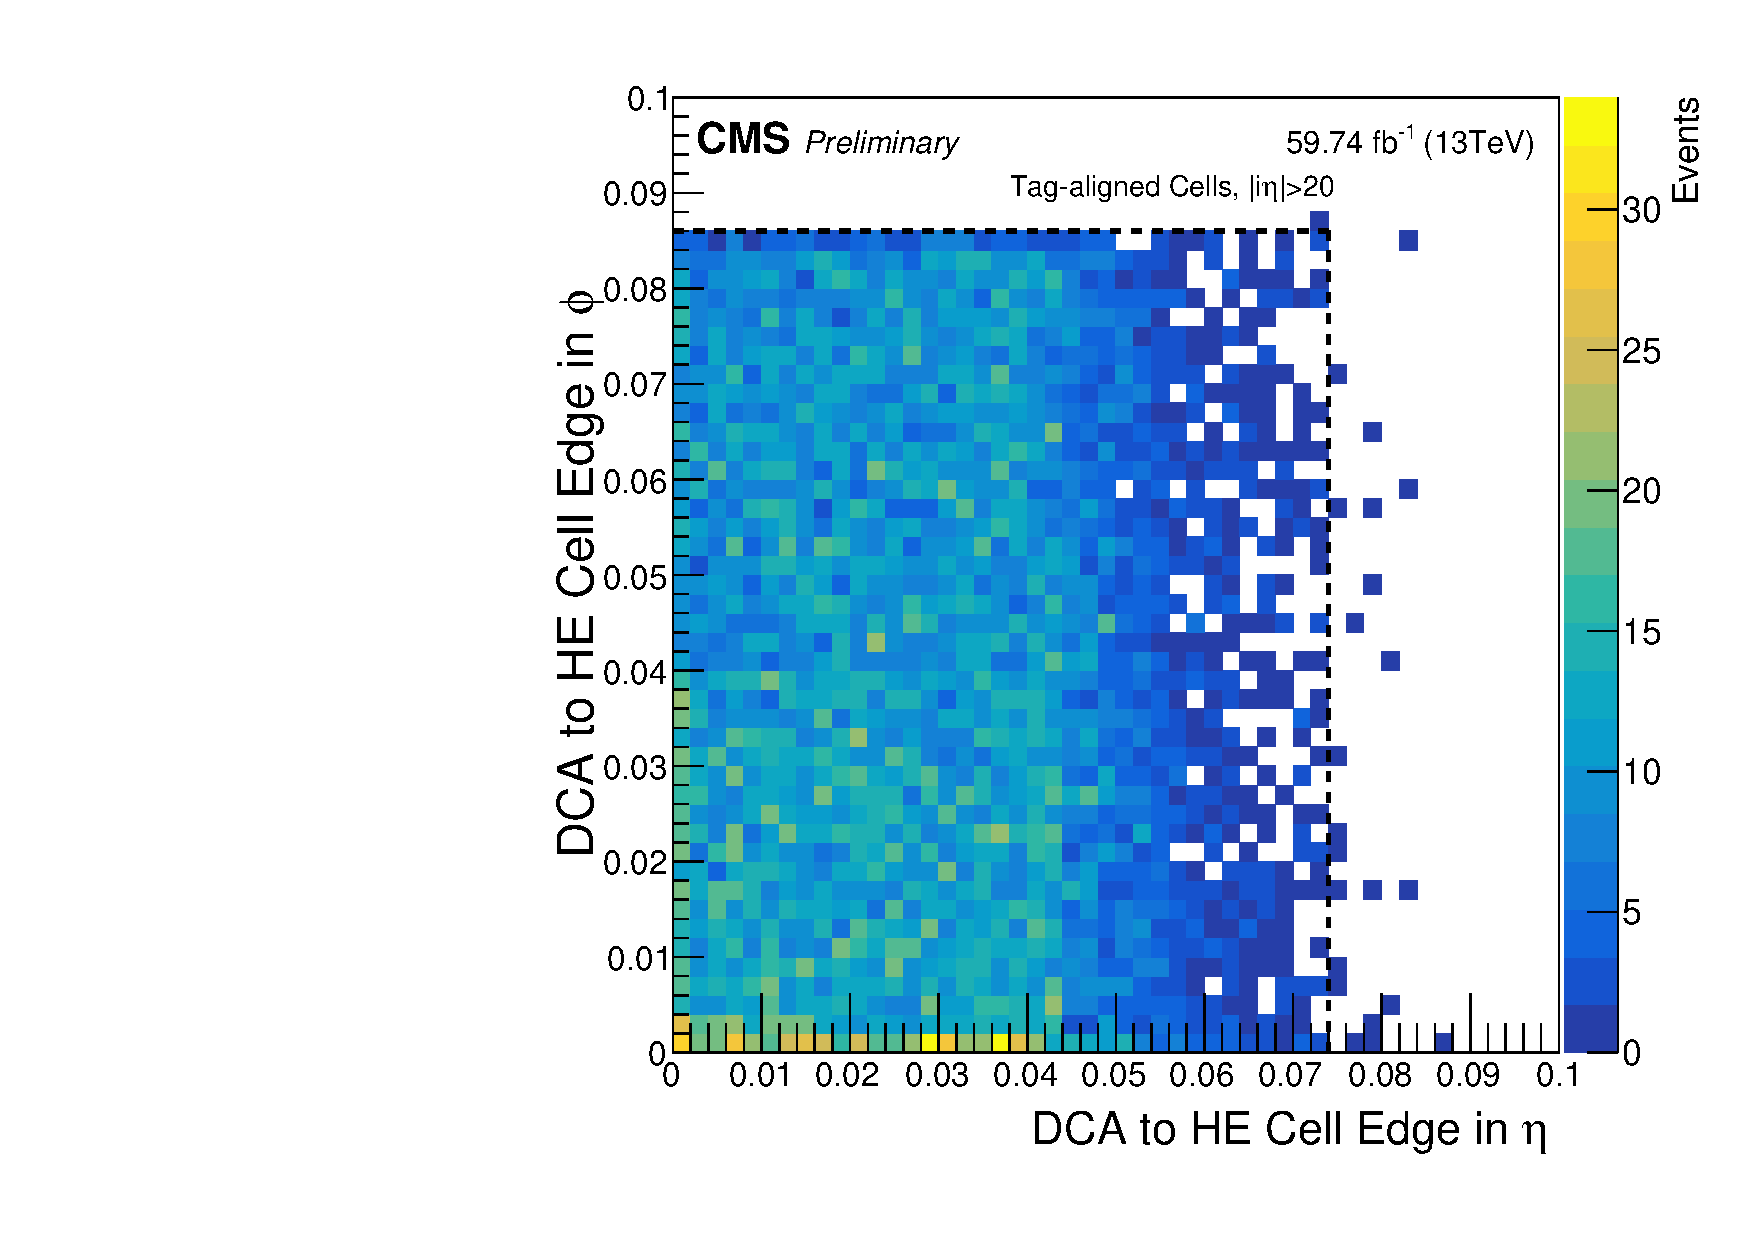
\includegraphics[width=0.45\textwidth]{figures/HEEdgeDistance_all.pdf}
        \hspace{0.01\textwidth}
        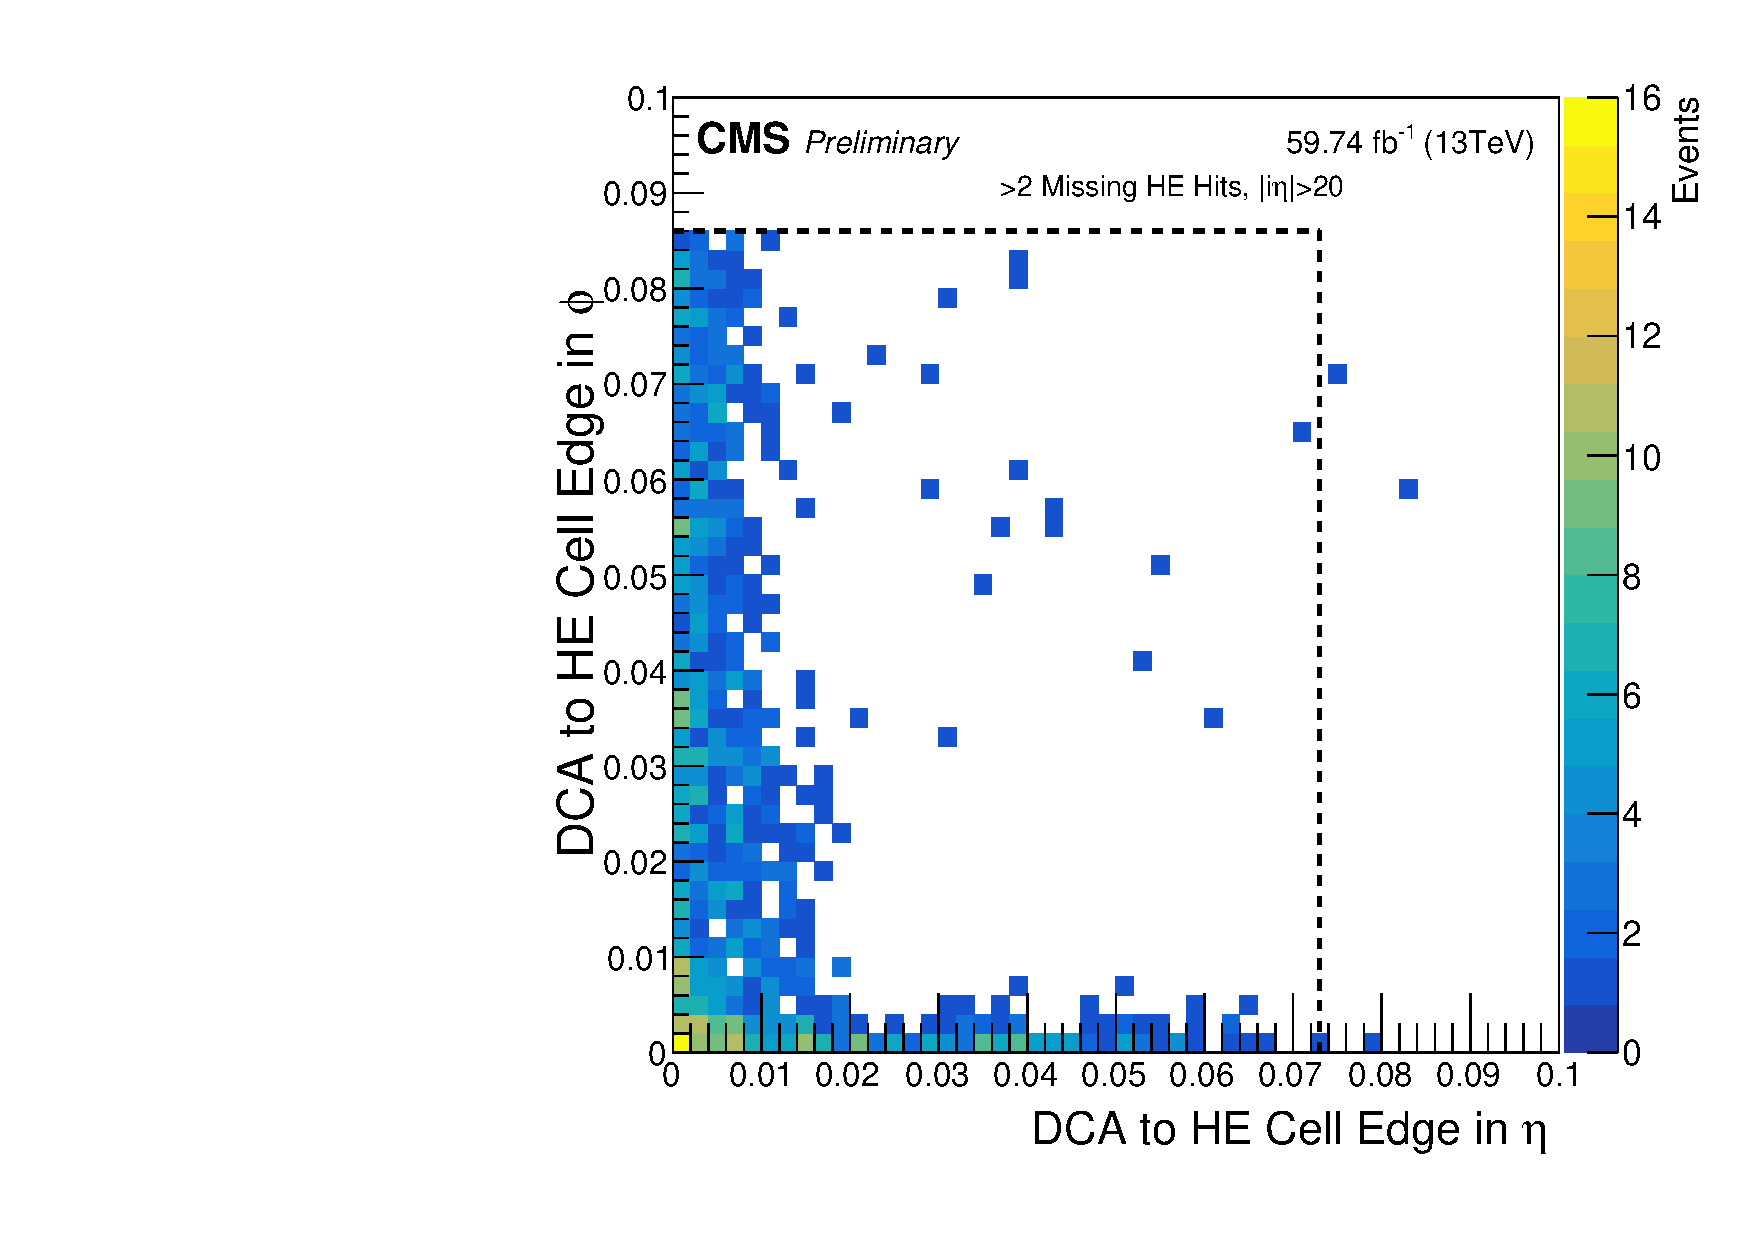
\includegraphics[width=0.45\textwidth]{figures/HEEdgeDistance_multMissing.pdf}

        \caption[Muon distances to HE cell edges]{The distance of closest approach (DCA) to any HE cell edge for tagging muons used to validate HE hits. Events with more than two missing hits (right) are clustered near the edges of HE cells, while the overall distribution of tracks is spread evenly across the cell size. The vertical splitting reflects the two different cell sizes in the detector, with the cell size in each region represented by the dotted line. The cell size is not observed to significantly change the size of the $\Delta\eta$ and $\Delta\phi$ regions with many missing hits.}
        \label{fig:cellEdges}
\end{figure}

Anomalous low-hit events that are produced by misalignment between the HE and the tracker in reconstruction will have correlations between the probe track trajectory and the $\Delta\eta$ and $\Delta\phi$ to cell edges which produce significant missing hits. 
To study these correlations, the $\eta$ edge and $\phi$ edge events are first categorized using requirements of $\mid\Delta\phi\mid$ $<$0.004 and $\mid\Delta\eta\mid$ $<$0.016, respectively. 
By defining events with probe tracks aligned with tagging muons which are not near $\phi$ edges as well as similar tag-aligned events which are not near $\eta$ edges, the two patterns can be separated and correlations in the cell edge distances which produce many missing hits and the probe track trajectory can be found. 
The $\Delta\phi$ from the probe track to the nearest HE cell edge in non-$\eta$-edge events with multiple missing hits is shown as a function of $\phi$ in \Cref{fig:phiEdgeCorr}, and the $\Delta\eta$ from the probe track to the nearest HE cell edge in non-$\phi$-edge events with multiple missing hits is shown as a function of $\eta$ for both endcaps in \Cref{fig:etaEdgeCorr}.

\begin{figure}[htpb]
    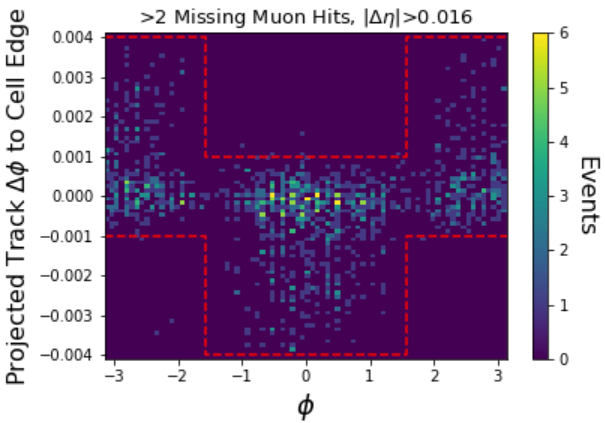
\includegraphics[width=0.45\textwidth]{figures/phiEdgeEventsData.png} 
    \centering
	\caption[$\phi$ edge correlations in missing HCAL muon hits.]{The minimum $\Delta\phi$ to any HE cell edge and the probe track $\phi$ trajectory for tag-aligned probe tracks with multiple missing hits. A sinusoidal dependence on the region with significant missing hits is observed, which is consistent with a relative shift in y between the HCAL and the tracker between data and reconstruction. The region outlined with a dashed red line indicates 'on-edge' events in $\phi$.}
    \label{fig:phiEdgeCorr}
\end{figure}

\begin{figure}[htpb]
    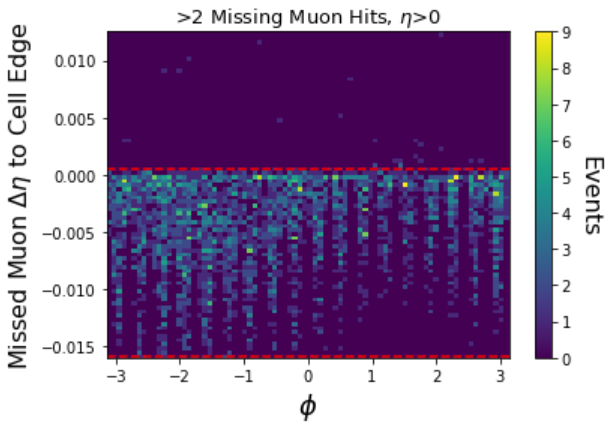
\includegraphics[width=0.45\textwidth]{figures/posEtaEdgeEventsData.png} 
    \hspace{0.01\textwidth}
    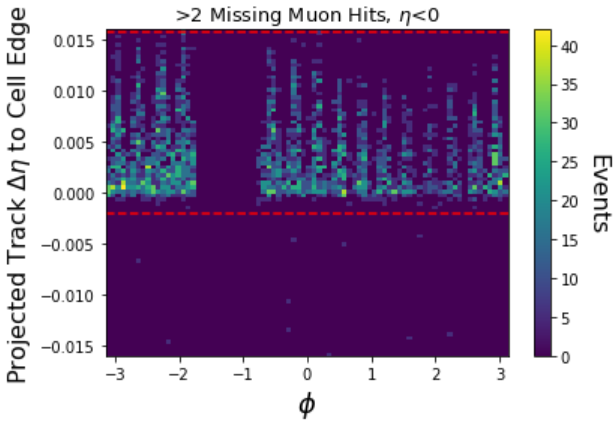
\includegraphics[width=0.45\textwidth]{figures/negEtaEdgeEventsData.png}
    \centering
	\caption[$\eta$ edge correlations in missing HCAL muon hits.]{The minimum $\Delta\eta$ to any HE cell edge and the probe track $\phi$ trajectory for tag-aligned probe tracks with multiple missing hits in the positive (left) and negative (right) HCAL endcaps. The events with multiple missing hits have a strong dependence on the sign of $\Delta\eta$ to the missing cell edges. The regions outlined with dashed red lines indicate 'on-edge' events in $\eta$.}
    \label{fig:etaEdgeCorr}
\end{figure}

Strong correlations are observed between the location of the projected tracks and the cell edge distances which produce missing hits, indicating that these 'missing hit' events are primarily caused by differences in the simulated and real position of the HE detector.
To account for these correlations, the 'on-edge' requirements are chosen to be dependent on the probe track trajectory as well as the cell edge distance. 
Probe tracks with $\eta<$0 are designated as on-edge in $\eta$ if -0.002$<\Delta\eta<$0.016, and probe tracks with $\eta>$0 are designated as on-edge in $\eta$ if -0.016$<\Delta\eta<$0.002.
Probe tracks with $|\phi|>\pi$/2 are designated as on-edge in $\phi$ if -0.001$<\Delta\phi<$0.004, and probe tracks with $|\phi|<\pi$/2 are designated as on-edge in $\phi$ is -0.004$<\Delta\phi$<0.001.

Events which are on-edge in $\eta$, $\phi$, or both are excluded from the partial disappearance region due to the significant differences observed between data and MC in the individual HE hits, which are necessary in that region to remove soft SM Bremsstrahlung backgrounds.
In complete disappearance events, the HCAL hits are implemented using sums of all HCAL cells within a $\Delta$R cone of 0.3, which is sufficiently large to include all adjacent cells and is not significantly affected by this misalignment.

After removing the on-edge events, small variations in the energy of muons in HE are still observed, as shown in \Cref{fig:nonEdgeHEEnergy}. 
To correct for these differences, event weights are derived for each depth in HE as a function of the energy in that depth based on the difference observed between DY MC and data.
The total re-weighting factor is calculated as the product of the weight in each depth that the track is expected to traverse.
To avoid potential differences in the simulated zero-suppression thresholds which may cause significant changes in events with very low HE energy, all HE hits with reconstructed energy below \SI{0.1}{\giga\eV} are set to zero.
The resulting scale factors for simulated DY events are shown in \Cref{fig:HESFs}.

\begin{figure}[htbp]
	\centering
	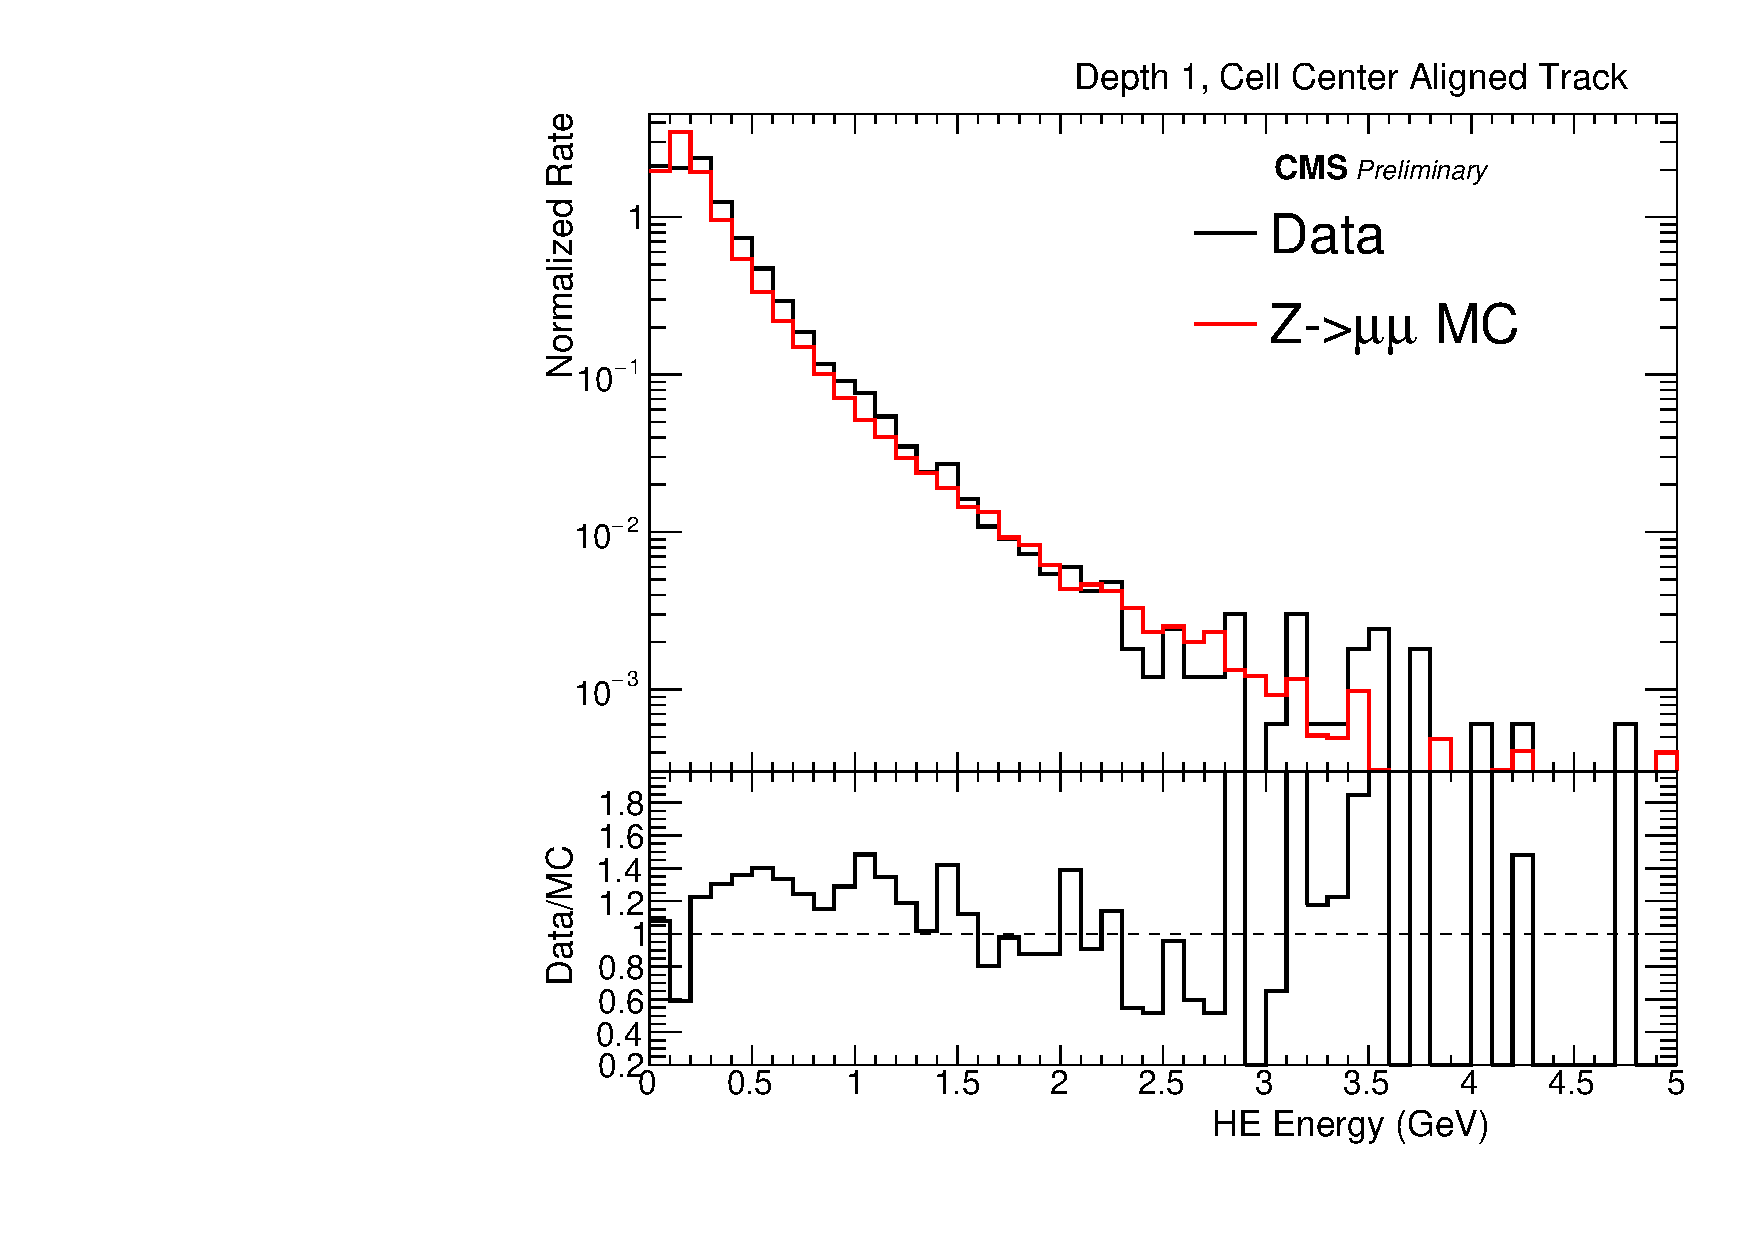
\includegraphics[width=0.45\textwidth]{figures/hcalE_depth0.pdf}
        \hspace{0.01\textwidth}
        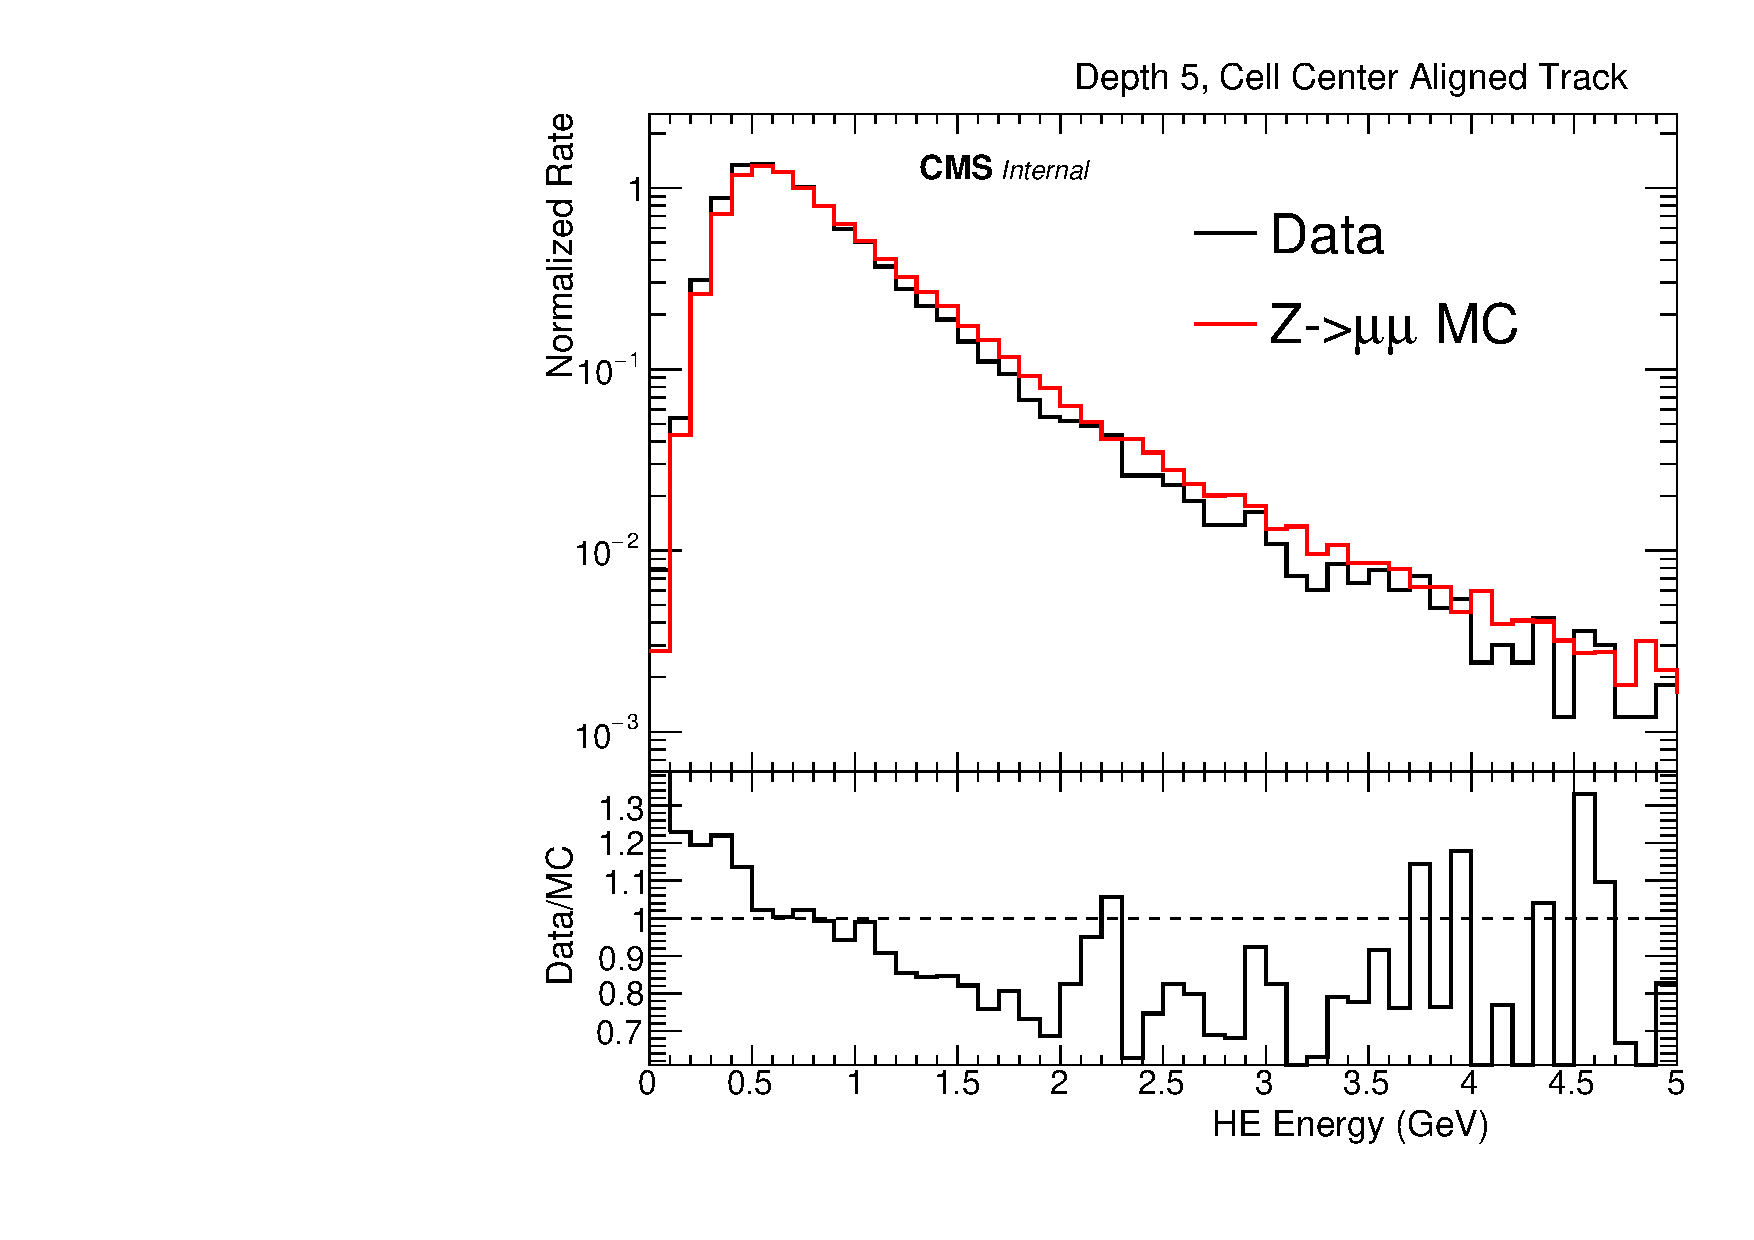
\includegraphics[width=0.45\textwidth]{figures/hcalE_depth4.pdf}
	\caption[Center-Aligned HE Energy]{The HE energy in two depths along tag-aligned muons for events not near the edge of HE cells. After removing the tracks with trajectories near cell edges, the excess in data events for events with very low energy is greatly reduced, and the ratio of simulated and data events from these comparisons is later applied as a correction factor to DY MC.} 
        \label{fig:nonEdgeHEEnergy}
\end{figure}

\begin{figure}[htbp]
	\centering
	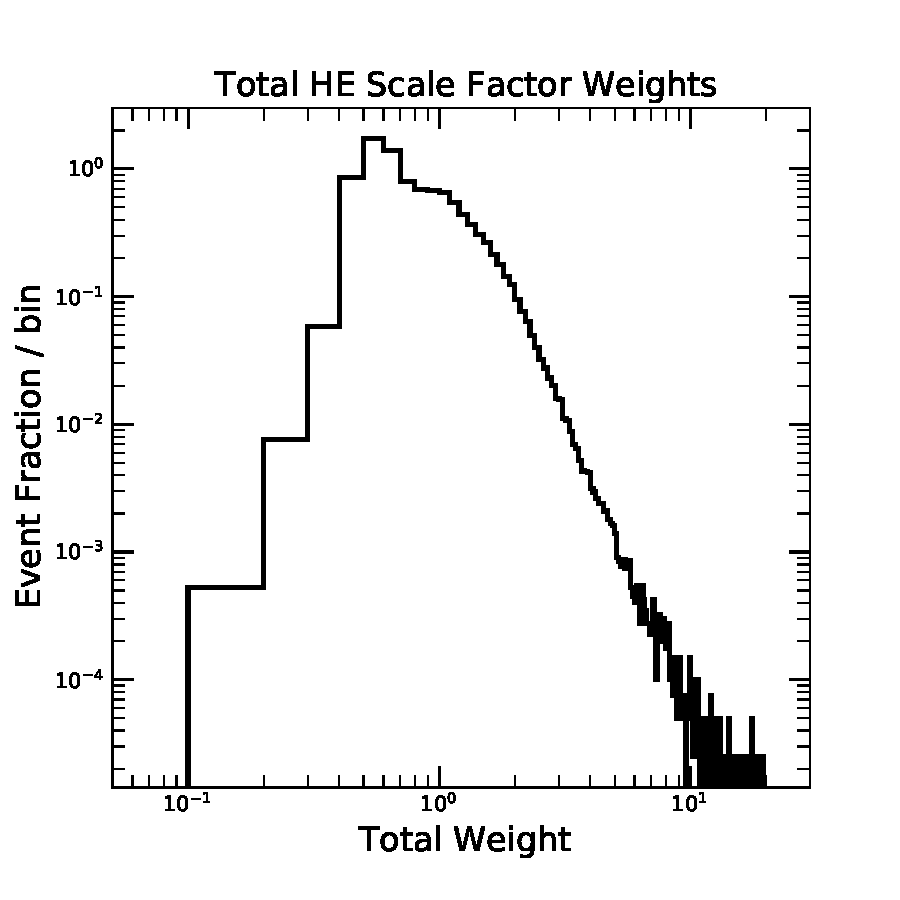
\includegraphics[width=0.45\textwidth]{figures/totalHEWeights.pdf}
	\caption[Applied HCAL Scale Factors]{The weights applied to simulated DY events resulting from the individual HE depth corrections. The corrections are derived iteratively for each successive depth, and the resulting weight is the product of the weights from each HE depth along the probe trajectory.} 
        \label{fig:HESFs}
\end{figure}

\subsection{Pileup Correction}
Generation of simulated events generally occurs concurrently with the operation of the experiment, when the exact pileup distribution is not well known.
As a result, estimates of the distribution of pileup vertices are used during the initial MC generation which may be significantly different from the real conditions within the detector. 
After data taking is complete and the resulting pileup distribution is measured, the simulated events are re-weighted to recreate the observed pileup.
Pileup events may produce particles which are mistakenly identified as muons or are in the vicinity of a probe track and cause it to fail isolation requirements, so potential differences in the number of pileup particles between data and MC could change the efficiency of selecting disappearing tracks and thus impact the expected signal strength.

To perform this re-weighting, histograms of the amount of pileup observed in data are divided by those used to generate the MC samples to find the weight for each potential number of pileup interactions (\Cref{fig:pileup}).
The number of pileup interactions used for this re-weighting is not directly the number of pileup vertices in the event, which is dependent on the vertex reconstruction efficiency in the event and can introduce large systematic errors and biases.
Instead, the rate of pileup is determined from the product of the total inelastic proton-proton cross section in CMS and the instantaneous luminosity, defined as the luminosity measured using dedicated detectors over each 23 second period ("lumisection") in CMS.
The amount of pileup in each event is then found by dividing this rate by the collision frequency.

As a result of this process, the measured pileup has a systematic uncertainty produced by uncertainty on the measured total proton-proton inelastic cross section as well as the instantaneous luminosity. 
These effects are included as a pileup re-weighting uncertainty by varying the product of cross section and luminosity by one standard deviation in each direction.
For the pileup calculation, the nominal total inelastic cross section of $\sigma_{pp}=$\SI{69.2}{\milli\barn} was used with an overall uncertainty of $\pm4.6\%$~\cite{pileupCx}.

\begin{figure}[ht]
	\centering
	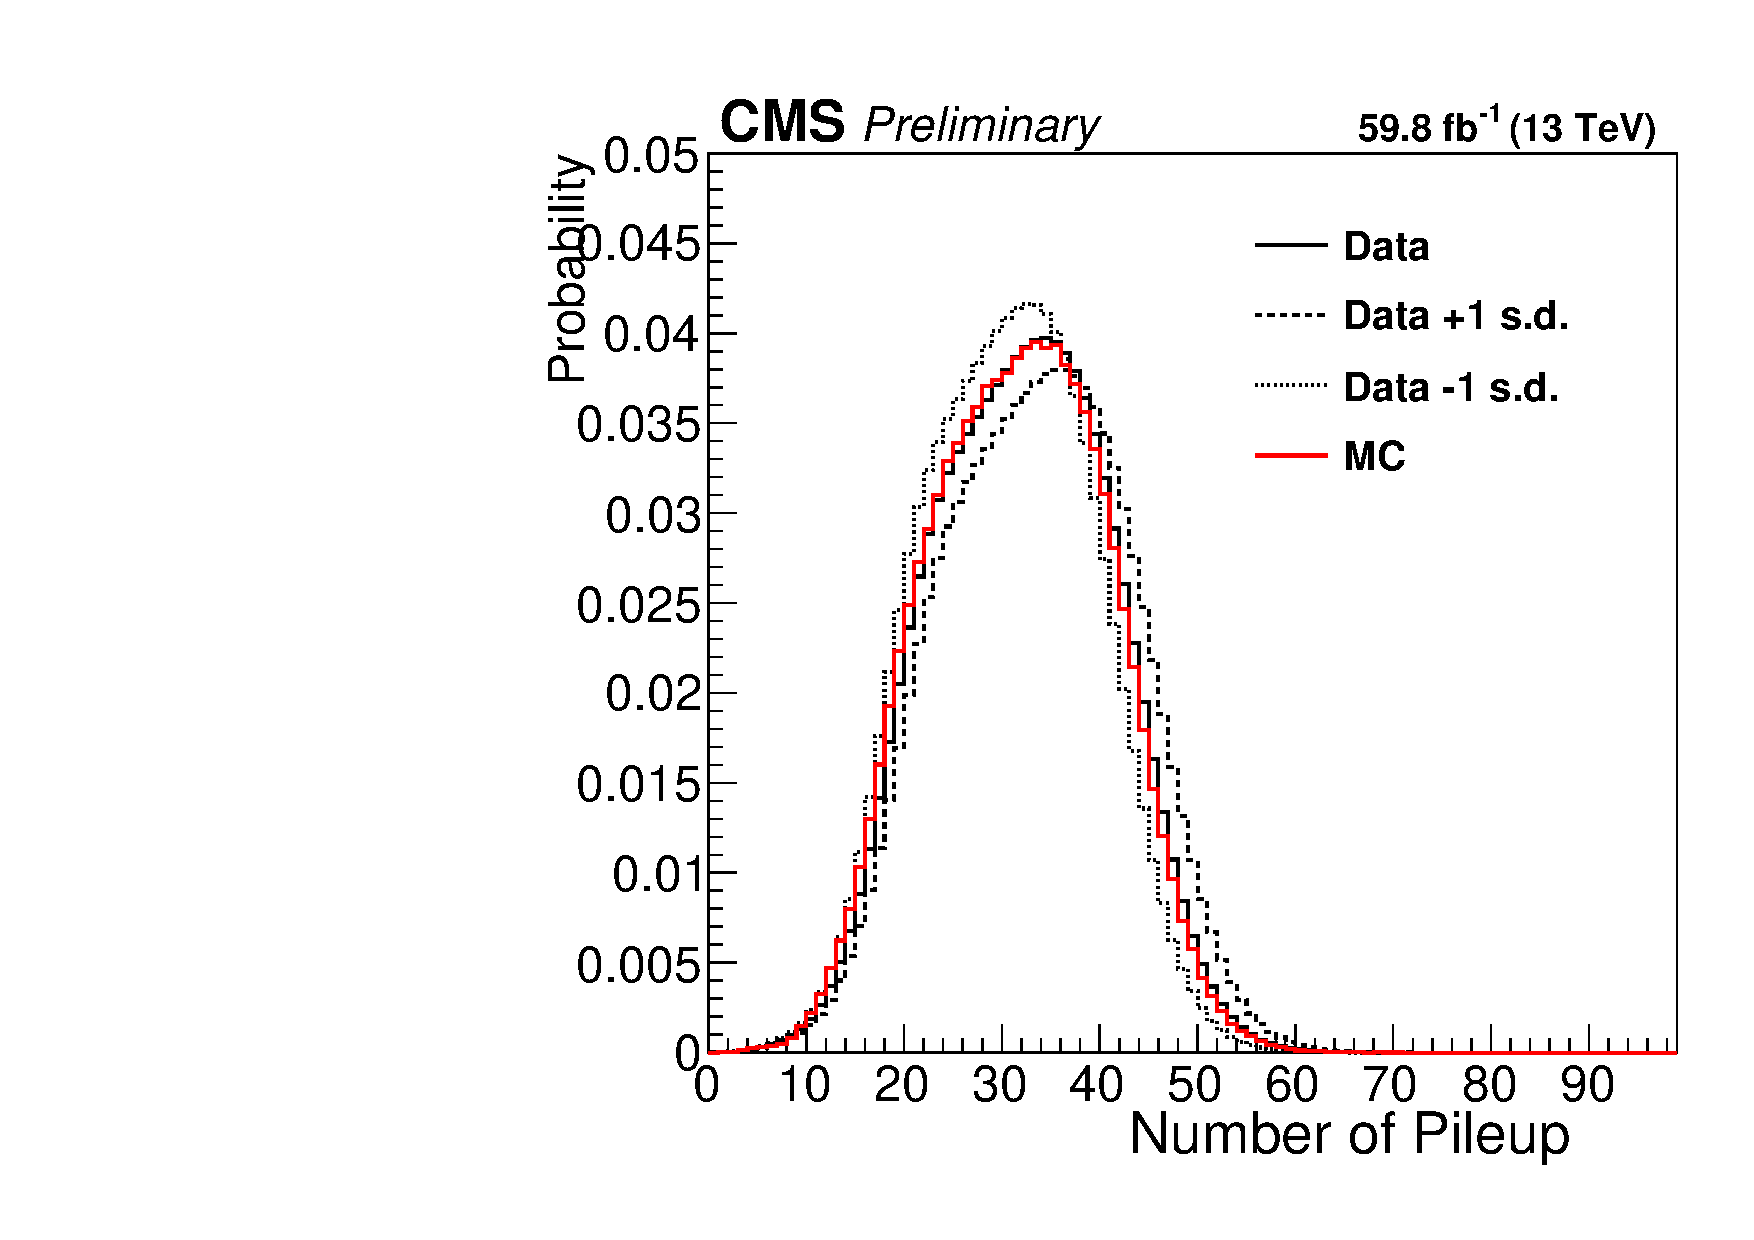
\includegraphics[width=0.45\textwidth]{figures/PileupDists.pdf}
	\hspace{0.01\textwidth}
	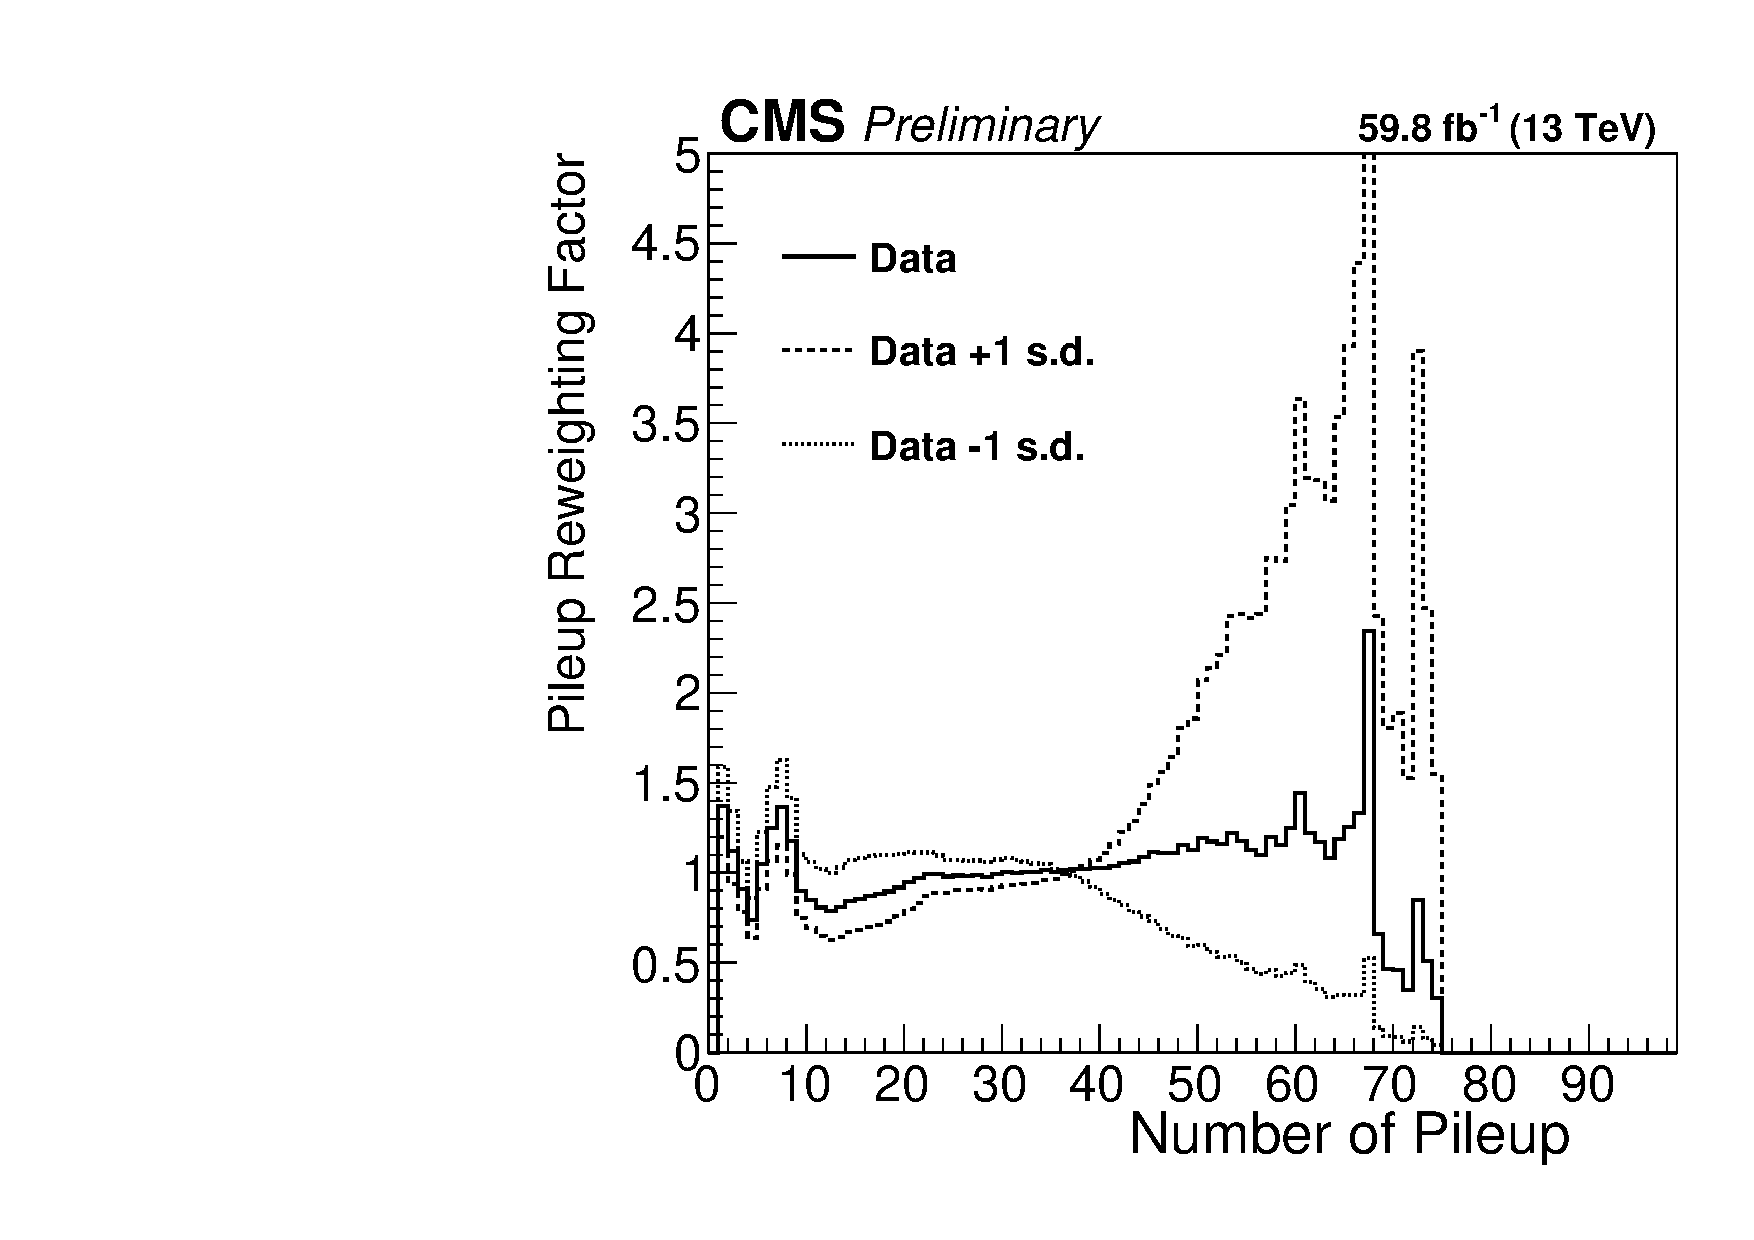
\includegraphics[width=0.45\textwidth]{figures/PileupRatioDists.pdf}
        \caption[Pileup Re-weighting Histograms]{The number of pileup interactions in data and simulation(left) and the pileup re-weighting factors (right) derived from their ratio.}
        \label{fig:pileup}
\end{figure}

%%%%%%%%%%%%%%%%%%%%%%%%%%%%%%%%%%%%%%%%%%%%%%%%%%%%%%%%%%%%%%%%%%%%%%%%%%%%%%%%
